\chapter{Calibración utilizando acoplamientos mútuos}
\label{ch:convertidores}
\lhead{\emph{Calibración utilizando acoplamientos mútuos}}
%\lhead{\emph{Celdas de combustible}}

\section{Calibración utilizando acoplamientos mútuos}

El método que utiliza los acoplamientos mútuos toma ventaja del acoplamiento mútuo inherente de un arreglo transmitiendo 
y recibiendo entre elementos adyacentes. Para llevar a cabo dicho método, este tipo de antenas debe cumplir un 
requerimiento muy importante que es poder transmitir con un elemento y simultáneamente recibir con otro. 
Ordinariamente, este requerimiento implica separar las redes de transmisión y recepción \cite{Gao2001}. Para antenas que no 
cumplen la separación de la redes de transmisión y recepción se puede transmitir en una polarización y recibir en otra. A 
su vez, para evitar que los elementos que no conforman parte del lazo activo de calibración interfieran, inyectando ruido en 
las redes de transmisión y/o recepción, se los debe poder configurar en modo alta impedancia (en este modo no se transmite ni recibe señal). 
En la figura \ref{fig:mutual_general} se puede observar un ejemplo.



\begin{figure}[H]
 \centering
 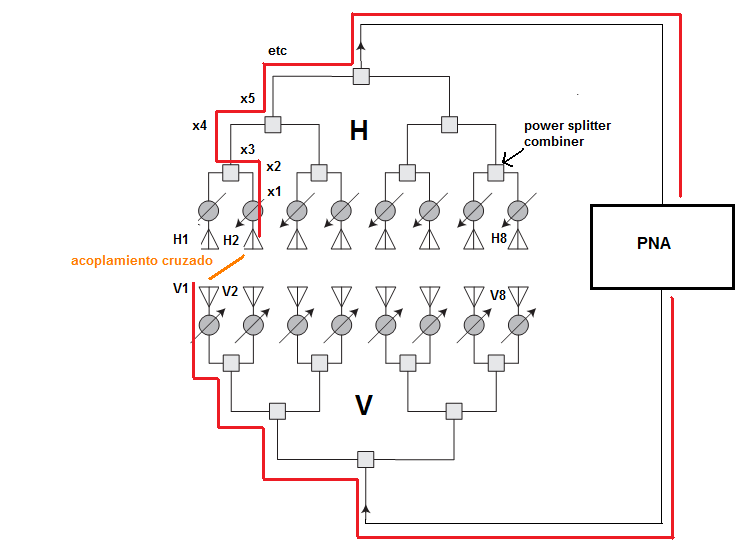
\includegraphics[width=9cm]{gfx/mutualCouplingExample.png}
 \caption{Ejemplo de calibración utilizando acoplamientos mútuos, transmitiendo en la polarización V y recibiendo en H}
 \label{fig:mutual_general}
\end{figure}

En la figura \ref{fig:mutual_general} se puede observar un ejemplo en donde se transmite utilizando el elemento $e_1$ en 
polarización horizontal (H) y se recibe con el elemento $e_0$ en polarización vertical (V). Si se repite el proceso 
secuencialmente con todos los elementos de recepción y luego con todos los elementos de transmisión, se puede determinar a 
priori tanto la potencia de transmisión como la de recepción y lo que atenúa cada acoplamiento mútuo.

Como un primer paso, se determina que la cantidad de incógnitas que tiene una antena de $m$ elementos por $n$ paneles. Como 
se puede transmitir y recibir en dos polarizaciones (H y V), la antena cuenta con $4MN$ incógnitas de RFDN (2 por Tx en H/V y 
otras 2 por Rx en H/V). A su vez, en el apéndice \ref{AppendixA} se realiza el cálculo de la cantidad de acoplamientos mutuos
que posee una antena polarimétrica, particularmente, la ecuación \ref{eq:amountMutCoupling} muestra la cantidad de 
incógnitas, que, para este caso, resulta ser de $MN(MN-1)/2$. Totalizando en $MN(MN + 7)/2$ incógnitas.

Asumiendo que se transmite de a un RM por lazo de calibración, a priori, se dispone de un máximo de $(MN)^2$ ecuaciones por
polarización a transmitir. Totalizando en $2(MN)^2$. Para que el sistema tenga solución, la cantidad de ecuaciones debe ser 
mayor a la de las incógnitas, por lo tanto, la cantidad mínima de elementos radiantes es de

$$
\begin{aligned}
	2(MN)^2 &\ge  \dfrac{MN(MN + 7)}{2} \\
	4MN &- MN \ge7 \\
	MN &\ge \dfrac{7}{3}
\end{aligned}
$$

Por lo tanto, como $M$ y $N$ son números enteros, con que la antena tenga tres o más elementos radiantes, ya se puede utilizar el método.

La herramienta matemática utilizada para resolver el sistema de ecuaciones es el de los cuadrados mínimos, 
\todo[inline]{ver apéndice tal }, con el cual se obtiene la aproximación que tenga menor error cuadrático medio. 

Ante la posibilidad que no siempre se cuente con el tiempo necesario para generar todos los lazos de calibración necesarios 
para calibrar la antena en el modo presentado, tres modalidades serán presentadas para este método. 

\begin{itemize}
	\item \textbf{Modo completo:} En esta modalidad no solo se estima la ganancia en transmisión y recepción en ambas 
		polarizaciones (H y V), sino que también se determinan los acoplamientos mutuos de la antena. La cantidad de ecuaciones necesarias es 
		de $MN(MN + 7)/2$.
	\item \textbf{Modo rápido:} En esta modalidad se estima la ganancia en transmisión y recepción em ambas polarizaciones
		(H y V) utilizando el valor guardado de la planitud de la antena calculado previamente. La cantidad de ecuaciones necesarias
		es de $4MN$.
	\item \textbf{Modo planitud ideal:} Esta modalidad es igual al modo rápido, asuminedo que la antena es perfectamente plana. 
		La cantidad de ecuaciones necesarias es de $4MN$.
\end{itemize}




\subsection{Método}

Asumiendo que se transmite desde el elemento $e_m$ y se recibe desde el $e_n$, la función de transferencia del lazo de 
calibración está compuesta por:

\begin{itemize}
	\item La configuración de atenuación y defasaje de los defasadores y atenuadores, tanto de transmisión como de recepción, 
		denotados como $w_{Tm}(i)$ y $w_{Rn}(j)$, donde $i$, $j$ son las diferentes posibles configuraciones. 
	\item La atenuación y defasaje combinados por los cables, conectores, divisores y combinadores de potencia, módulos radiantes
		y defasadores, denotados como $u_{Tm}$ y $u_{Rn}$. 
	\item El acoplamiento mútuo entre los elementos participantes, denotado como $C_{m, n}$.
\end{itemize}
		
Por lo tanto, la función de transferencia completa resulta,

\begin{equation}
	C^{'}_{m,n} = w_{Tm} u_{Tm} C_{m,n} w_{Rn} u_{Rn}
	\label{eq:transfer_mn}
\end{equation}

Si se transmite con el mismo elemento, $e_m$, pero se recibe con otro, $e_{n + 1}$, la transferencia resulta

\begin{equation}
	C^{'}_{m,n + 1} = w_{Tm} u_{Tm} C_{m,n + 1} w_{Rn + 1} u_{Rn + 1}
	\label{eq:transfer_mn1}
\end{equation}

Tomando la relación de ambas transferencias \ref{eq:transfer_mn} y \ref{eq:transfer_mn1},

\begin{equation}
	W^{'}_{Rn,n + 1} = \dfrac{C^{'}_{m,n}}{C^{'}_{m,n + 1}} = \dfrac{C_{m,n} w_{Rn} u_{Rn}}{C_{m,n + 1} w_{Rn + 1} u_{Rn + 1}}
\end{equation}

\todo{seguramente hay que sacar este texto de aca y ponerlo en la introducción del método y posiblemente en las hipotesis}
Se asume que el valor del acoplamiento depende de dos factores a saber. El primero es por comunicar los elementos utilizando
polarizaciones cruzadas, y dicha atenuación es constante para cualquier elemento. El segundo, es debido a la atenuación y 
defasaje de la señal que viaja en el vacío, por lo tanto, depende exclusivamente de la distancia que hay entre los elementos
a comunicar.

Ahora, si se transmite con $e_{n+1}$ y se recibe con el elemento $e_{n+2}$, la relación resultante es,

\begin{equation}
	W^{'}_{Rn + 1,n + 2} = \dfrac{C^{'}_{m,n+1}}{C^{'}_{m,n+2}} = \dfrac{C_{m,n+1} w_{Rn+1} u_{Rn+1}}{C_{m,n + 2} w_{Rn + 2} u_{Rn + 2}}
\end{equation}

Ahora, si se recibe con el elemento $e_{n+2}$ transmitiendo con $e_n$, la relación resultante es,

\begin{equation}
	W^{'}_{Rn,n + 2} = \dfrac{C^{'}_{m,n}}{C^{'}_{m,n + 2}}\cdot\dfrac{C^{'}_{m,n+1}}{C^{'}_{m,n+1}} = W^{'}_{Rn,n+1}\cdot W^{'}_{Rn+1,n + 2}
\end{equation}

Generalizando, se pueden obtener todos los lazos de calibración en función de uno se obtiene,
\todo{puta madre.... ajajaj, no recuerdo cual es la mierda del producto}

\begin{equation}
	W^{'}_{R0,k} = W^{'}_{Rn,n+1}\cdot W^{'}_{Rn+1,n + 2}
	\label{eq:rx_cal}
\end{equation}

Si se realiza la misma deducción, pero en vez de transmitir siempre con el mismo elemento, se lo utiliza para recibir, se obtiene 

\todo{puta madre.... ajajaj, no recuerdo cual es la mierda del producto, poner y separar las dos productorias de cij y u,v ij}
\begin{equation}
	W^{'}_{T0,k} = W^{'}_{Rn,n+1}\cdot W^{'}_{Rn+1,n + 2}
	\label{eq:tx_cal}
\end{equation}

Analizando las ecuaciones \ref{eq:tx_cal} y \ref{eq:rx_cal}, dos conclusiones inmediatas se deducen. La primera es que el 
resultado no es único, por lo tanto, el método no puede devolver la ganancia absoluta de transmisión, recepción y de
acoplamientos mútuos, solamente la ganancia relativa entre dichos elementos. La segunda, es que el sistema tiene dos grados 
de libertad, en otras palabras, para poder obtener la ganancia absoluta de todo el sistema, es necesario agregar dos ecuaciones
más que definan un único valor pertenenciente a dos de los tres conjuntos de incógnitas.

Si se asumen conocidos los acoplamientos mútuos o se reutilizan de una calibración anterior, las ecuaciones \ref{eq:tx_cal} 
y \ref{eq:rx_cal} se simplifican, logrando que la cantidad de incógnitas se reduzca habilitando de esta forma los métodos
rápidos y de planitud ideal.

\todo{Poner las ecuaciones simplificadas y ver en el paper si pusieron algo mas como para robar muejeje}
\todo{poner las estrategias en este caso}

Como es necesaria una menor cantidad de lazos de calibración, se realizaron distintas estrategias para obtener una solucion de 
compromiso entre la cantidad de lazos de calibración necesarios para poder utilizar el método y la cantidad de ecuaciones 
redundantes que le da robustez al resultado.


La ecuación \ref{eq:transfer_mn2} resulta en la relación que hay entre los caminos de recepción de los elementos $n$ y 
$n+1$. Si al elemento $e_m$ se lo utiliza para recibir y a los elementos $e_n$ y $e_{n + 1}$ para transmitir, la ecuación que se 
obtiene sirve para calibrar la antena en modo transmisión.

\begin{equation}
	W^{'}_{Tn,n + 1} = \dfrac{w_{Tn} u_{Tn}}{w_{Tn + 1} u_{Tn + 1}}
\end{equation}

El cálculo previo sirve solamente para el caso donde se conoce el acoplamiento mútuo entre distintos elementos. Para el caso 
en que se desee obtener la planitud de la antena, es necesario trabajar de a pares de módulos radiantes como sigue. En la 
ecuación siguiente se transmite con el elemento $e_m$ y se recibe con el $e_n$.

\begin{equation}
	C^{'}_{m,n} = w_{Tm} u_{Tm} C_{m,n} w_{Rn} u_{Rn}
	\label{eq:transfer_mn22}
\end{equation}


Ahora, si se intercambian los roles, se recibe con el elemento $e_m$ y se transmite con el $e_n$, la transferencia resultante es,

\begin{equation}
	C^{'}_{n, m} = w_{Tn} u_{Tn} C_{n,m} w_{Rm} u_{Rm}
	\label{eq:transfer_nm2}
\end{equation}

Tomando la relación de ambas transferencias \ref{eq:transfer_mn22} y \ref{eq:transfer_nm2},

\begin{equation}
	W^{'}_{Rn,m} = \dfrac{C^{'}_{m,n}}{C^{'}_{n, m}} = \dfrac{w_{Tm} u_{Tm} C_{m,n} w_{Rn} u_{Rn}}{w_{Tn} u_{Tn} C_{n,m} w_{Rm} u_{Rm}}
	\label{eq:transfer_mn3}
\end{equation}

Y, como son las mismos elementos, el acoplamiento mútuo se cancela, resultando en.

\begin{equation}
	W^{'}_{Rn,m} = \dfrac{C^{'}_{m,n}}{C^{'}_{n, m}} = \dfrac{w_{Tm} u_{Tm} w_{Rn} u_{Rn}}{w_{Tn} u_{Tn} w_{Rm} u_{Rm}}
	\label{eq:transfer_mn4}
\end{equation}
\todo[inline]{hasta aca llego con el tema para determinar la planitud de la antena}

\todo{ahora tengo que continuar con el metodo normal}

El Modo Completo requiere una enorme cantidad de mediciones para poder obtener resultados, por lo tanto, es necesario 
complementarlo con un modo más rápido que no necesariamente obtenga todos los parámetros. Aprovechando que las variaciones 
mecánicas son muchisimo más lentas que las eléctricas, entre calibración y calibración, se asume que los acoplamientos se 
mantienen constantes. De esta forma, se calibra la antena utilizando el método rápido, en el cual se reutilizan los $C_{i, j}$. 

Si la distancia entre los elementos $e_m$ y $e_n$ es la misma que la referente a los elementos $e_m$ $e_{n+1}$, o sea 
$d_{m,n} = d_{m,n+1}$, resulta que $C_{m,n} = C_{m, n + 1}$, logrando simplificar la ecuación \ref{eq:transfer_mn1}.

\begin{equation}
	W^{'}_{Rn,n + 1} = \dfrac{w_{Rn} u_{Rn}}{w_{Rn + 1} u_{Rn + 1}}
	\label{eq:transfer_mn2}
\end{equation}

La ecuación \ref{eq:transfer_mn2} resulta en la relación que hay entre los caminos de recepción de los elementos $n$ y 
$n+1$. Si al elemento $e_m$ se lo utiliza para recibir y a los elementos $e_n$ y $e_{n + 1}$ para transmitir, la ecuación que se 
obtiene sirve para calibrar la antena en modo transmisión.

\begin{equation}
	W^{'}_{Tn,n + 1} = \dfrac{w_{Tn} u_{Tn}}{w_{Tn + 1} u_{Tn + 1}}
\end{equation}


\todo{terminar diciendo que se programó el modo planitud ideal, porque iba mas alla del objeto de la tesis con las ecuaciones pertinentes}

\subsection{Problemas y limitaciones}


Una de las grandes ventajas de este método frente al método anterior es que no requiere hardware extra, logrando así 
disminuir la complejidad de la antena, de esta forma se la puede construir de una forma más compacta.

Tomando como $M$ la cantidad de filas de módulos radiantes por panel y $N$ la cantidad de paneles, las tres modalidades de 
este método son:

\begin{itemize}
	\item \textbf{Modo completo:} En esta modalidad no solo se estima la ganancia en transmisión y recepción en ambas 
		polarizaciones (H y V), sino que también se determina la planitud de la antena. La cantidad de ecuaciones necesarias es 
		de $MN(MN + 7)/2$.
	\item \textbf{Modo rápido:} En esta modalidad se estima la ganancia en transmisión y recepción em ambas polarizaciones
		(H y V) utilizando el valor guardado de la planitud de la antena calculado previamente. La cantidad de ecuaciones necesarias
		es de $4MN$.
	\item \textbf{Modo planitud ideal:} Esta modalidad es igual al modo rápido, asuminedo que la antena es perfectamente plana. 
		La cantidad de ecuaciones necesarias es de $4MN$.
\end{itemize}

El acoplamiento mútuo se lo modeliza como si fuese un cable pero con las propiedades de atenuación y defasaje de una onda en
el vacío. Las cuales son:

\todo{Poner que significa el alfa}
\begin{equation}
	c = \dfrac{e^{-2\alpha r}}{4\pi r^2}
\end{equation}

El modo planitud ideal cuenta con otra limitación que, si bien se asume que el acoplamiento mútuo es desconocido, se sabe que 
a distancias iguales dicho acoplamiento es el mismo. Por lo tanto, para calibrar una antena de cualquier topología solo se 
utilizan lazos de calibración simétricos con un módulo radiante común. Al restar ambos caminos, no solo se elimina el 
camino común, que puede ser la parte de transmisión o recepción, sino que también se elimina el acoplamiento mútuo.

Si el RM común se utiliza para transmitir la señal, se obtienen ecuaciones para calibrar la parte de recepción, en cambio, 
si se lo utiliza para recibir la señal, se calibra transmisión. La figura \ref{fig:ideal_strategy} esquematiza esta estrategia.

\begin{figure}[H]
 \centering
	\subfloat[]{	
		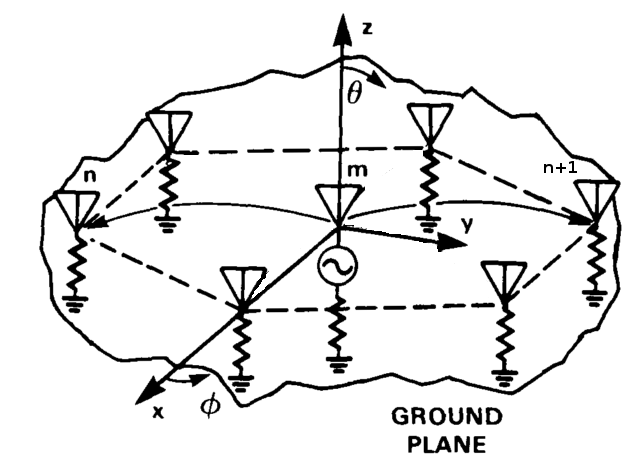
\includegraphics[width=5cm]{gfx/mutualRxCal.png}}
	\subfloat[]{	
		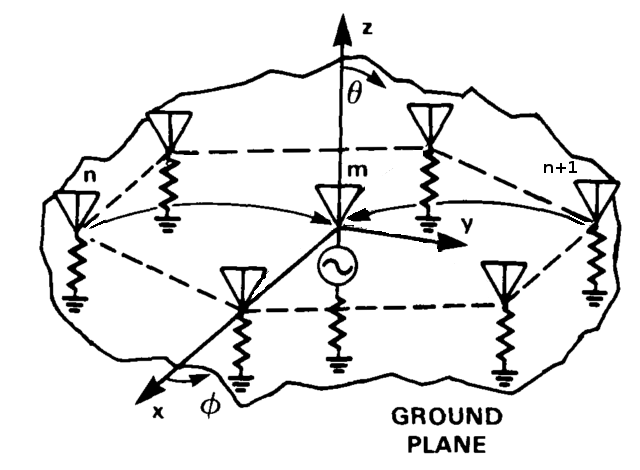
\includegraphics[width=5cm]{gfx/mutualTxCal.png}}
 \caption{estrategia de planitud ideal. (a) Calibra lazos de recepción, (b) Calibra lazos de transmisión}
 \label{fig:ideal_strategy}
\end{figure}




Aprovechando la realidad que las variaciones mecánicas son lentas frente a las variaciones eléctricas de los componentes,
no es necesario correr el método de calibración en su máxima caracterización dado que requiere demasiada cantidad de 
mediciones para determinar la planitud de la antena.


Referencias a utilizar: 
Shipley2000
Aumann1989
Gao2001 (este no esta tan copado, son puras formulas)
a calibration technique for active phased array antennas (no lo agregue aun a la bibliografia, je)
Practical faliure compensation in active phased antennas (ni lo lei, pero muy interesante que hacer para compensar algo quemado)


\todo{poner en algun lado que se sugiere para medir la fase de medir en un unico punto lo que defasa la antena punta a punta una unica vez y se lo carga al metodo}
\todo[inline]{esto es texto viejo... el capitulo 5 tiene lo mismo}
Una antena se calibra buscando que no solo todos los caminos de recepción atenúen y defasen exactamente lo mismo, sino que 
también sea un valor conocido. Para transmisión se busca lo mismo, con la salvedad que se puede modificar la fase de la 
señal que se emite en algunos RMs para modificar el lugar de apuntamiento de la antena.

Hay distintos factores que hacen que los componentes dejen de comportarse de forma nominal, por ejemplo se puede nombrar el
cambio de temperatura, el mero envejecimiento de los componentes al pasar el tiempo, que un mero cable se haya doblado más
de la cuenta, interferencias electromagnéticas, radiadas o conducidas, o entre distintos componentes, etc. 

Es importante que un patrón de antena posea los lóbulos secundarios lo más chicos posibles con respecto al lóbulo principal,
que el lóbulo principal sea lo más angosto posible, con esto se aumenta la resolución espacial. Un factor que ocurre es el 
de los targets ficticios.\todo{no se como se elimina}


\todo{poner que factores hacen que cambie la ganancia de los componentes para calibrar la antena}
\todo{poner que ocurre con el antnena pattern si no está correctamente calibrada, altura de lóbulos secundarios, ancho 
de lóbulo principal, pico del lóbulo principal, etc}

Para que el sistema tenga solución, la cantidad de ecuaciones debe ser mayor que la de incógnitas. Esta restricción solo 
se cumple si se calibra toda la antena en un solo paso (Tx y Rx en ambas polarizaciones) porque es el único caso en que 
cada acoplamiento mútuo aparezca más de una única vez. En caso contrario, habrían siempre más incógnitas que ecuaciones.

\todo{tener en cuenta que por ahora el requerimiento es que la antena sea totalmente plana}




\begin{comment}

Los convertidores conmutados son equipos de potencia utilizados para proveer una tensión regulada a partir
de una fuente de de energía eléctrica. Su característica principal es su gran eficiencia, comparados con otros
sistemas de conversión, gracias al mecanismo de conmutación en que están basados.

Existen varias configuraciones de circuitos de convertidores y en general se apoyan en tres topologías básicas cuya característica
les permite elevar o reducir la tensión, o bien realizar ambas. Estas configuraciones pueden ser modificadas
para adicionar algunos atributos como aislamiento eléctrico, múltiples niveles de tensión o la simplificación del accionamiento de las llaves electrónicas.

El principio operacional de los convertidores consiste en cambiar la estructura del circuito mediante
la activación de las llaves electrónicas, provocando un cambio en el comportamiento general del sistema.

Una de sus principales características es el control que se adopta en la apertura y cierre de las llaves electrónicas.
En general las señales de conmutación que ordenan su apertura o cierre, provienen de pulsos de ancho modulado (PWM)
cuya operación se controla a través de alguna referencia interna al dispositivo que las acciona.

Ciertos parámetros definen la operación de los convertidores de potencia, entre los más importantes se encuentran
la frecuencia de conmutación y el ciclo de trabajo correspondiente al tiempo de apertura de la llave activa, denotada por $D$.

La operación de los convertidores trabajando en régimen permanente se distingue en dos modos de operación que tienen
en cuenta el paso de corriente a través del inductor. Estos modos son los de \emph{conducción continua} y \emph{conducción discontinua}:
en el primero la corriente no se interrumpe y en el otro existe un intervalo en que se mantiene nula.

El rol de estos convertidores es de especial importancia para cualquier aplicación de las pilas de celdas de combustible 
debido a los cambios que sufre la tensión entregada ante cambios de carga, como se mostró en el cap. \ref{ch:modelo}.

En un SGH, estos convertidores son requeridos por tratarse de los dispositivos a través de los que se adaptan
los módulos de generación a la línea de distribución de energía. Para el proyecto de la construcción del SGH abordado se realizó
la construcción de una etapa de potencia para adaptar cierta pila de combustible al bus de tensión continua del sistema. Este dispositivo
fue hecho de modo que pudiera elevar la tensión entregada por la celda al nivel del la línea de distribución. Dado que el convertidor
cuenta con las especificaciones de diseño para operar con celdas de combustible fue elegido como soporte físico para el desarrollo del emulador.

Para la operación del emulador es necesario que el dispositivo de potencia pueda reducir la tensión, que es el comportamiento
general de las celdas de combustible al ser cargadas con cierta corriente. Por tanto se requirieron ciertos ajustes a nivel de \emph{software} 
y \emph{hardware} al convertidor ya diseñado para que tenga la capacidad de reducir la tensión en lugar de aumentarla. Las modificaciones 
realizadas sobre el elevador serán explicadas hacia el final del capítulo mientras que el control implementado será explicado en el cap. \ref{ch:control}.

Para la realización de los análisis siguientes se establecen las siguientes aproximaciones, que permiten simplificar
los cálculos con suficiente precisión:
\begin{itemize}
 \item El capacitor del filtro de tensión de salida es suficientemente grande para que se desprecie la variación
 de tensión a la salida.
 \item El inductor es suficientemente grande para que la corriente pueda ser considerada por tramos lineales.
 Este hecho permite establecer la siguiente aproximación:
 \begin{equation}
  \frac{di_L}{dt}\approx \frac{\Delta i_L}{\Delta t}\Rightarrow \Delta i_L=\frac{di_L}{dt}\Delta t
  \label{eq:aprox_corriente}
 \end{equation}
 Y la derivada representa la pendiente de la corriente en el subintervalo correspondiente.
 \item La corriente no sufre grandes variaciones debido a la presencia de elementos parásitos.
\end{itemize}

Este capítulo presenta las características generales de los convertidores utilizados y los parámetros utilizados para su control. 
El análisis se comienza por el dispositivo elevador original debido a que fue el soporte inicial. Luego se explicarán las características
técnicas particulares de cada convertidor utilizado.

A continuación se dará un explicación más detallada de los convertidores utilizados, su funcionamiento en régimen permanente en ambas
condiciones de conducción y el modelo dinámico que será utilizado para diseñar los controladores implementados.

\section{Convertidor elevador}
Este sistema de potencia, como indica su nombre, es usado para llevar la tensión de entrada a un nivel mayor. La
fig. \ref{fig:elevador} muestra un diagrama esquemático del circuito utilizado para la construcción de la etapa de potencia del SGH.
En ella se distingue la particularidad de la capacidad bidireccional de corriente que le confiere el uso de dos llaves de conmutación
en lugar de una, como sería en el caso más básico. Esta característica permite que el convertidor sea capaz de devolver potencia a la fuente y además
le da flexibilidad al modelo, cuya cualidad se aprovechó para cambiar la topología sin realizar mayores modificaciones.
Para que ello sea posible, el proceso de fabricación que se realiza para obtener las llaves colocadas en el equipo utilizado implica 
la formación de una juntura PN entre los terminales de \emph{drain} y \emph{source}, lo que permite que ambas llaves conduzcan en ambos
sentidos, ya sea con la corriente pasando a través del canal del transistor (si se encuentra activo) en un sentido o con la corriente pasando a través del
diodo mencionado en el otro sentido.

\begin{figure}[H]
 \centering
 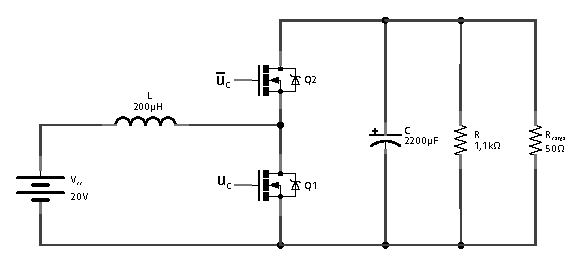
\includegraphics[width=10cm]{gfx/elevador.eps}
 \caption{Topología de un convertidor elevador de conducción bidireccional}
 \label{fig:elevador}
\end{figure}

\subsection{Operación en estado estacionario}
\label{sub:elevador_estacionario}
Una vez energizado y los transitorios extinguidos pueden analizarse las curvas eléctricas resultantes para obtener información acerca
de los parámetros de funcionamiento del convertidor y encontrar relaciones que serán útiles para el diseño del control. Esto puede hacerse 
cuando el convertidor opera en cualquiera de sus modos de funcionamiento.

\subsubsection{Modo de conducción continua}
Se procede a realizar una análisis del comportamiento del convertidor operando en modo de conducción continua (MCC). 
La fig. \ref{fig:elevador_CC} muestra las curvas genéricas de un convertidor utilizado funcionando en régimen permanente.

\begin{figure}
 \centering
 \subfloat[Tensión de inductor]{\label{fig:tension_inductor_elevador_MCC}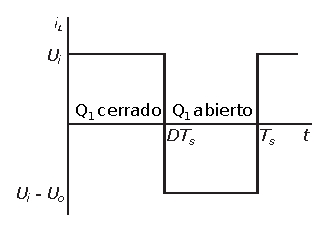
\includegraphics[width=5cm]{gfx/tension_inductor_elevador_MCC.eps}} \quad
 \subfloat[Corriente de diodo]{\label{fig:corriente_diodo_elevador_MCC}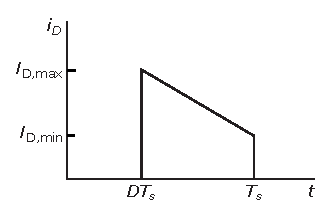
\includegraphics[width=5cm]{gfx/corriente_diodo_elevador_MCC.eps}} \\
 \subfloat[Corriente de inductor]{\label{fig:corriente_inductor_elevador_MCC}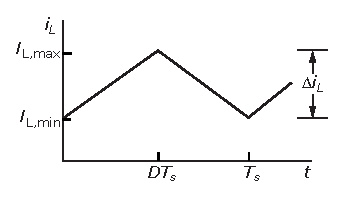
\includegraphics[width=5cm]{gfx/corriente_inductor_elevador_MCC.eps}} \quad
 \subfloat[Corriente de capacitor]{\label{fig:corriente_capacitor_elevador_MCC}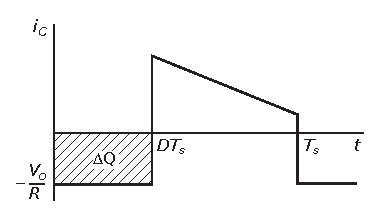
\includegraphics[width=5cm]{gfx/corriente_capacitor_elevador_MCC.eps}}
 \caption{Curvas de estado estacionario para el elevador operando en MCC}
 \label{fig:elevador_CC}
\end{figure}

Utilizando las curvas anteriores y conceptos elementales de la teoría de circuitos pueden obtenerse las relaciones que definen al funcionamiento
del elevador. El análisis realizado aquí considera también la presencia de algunos de los elementos parásitos que corresponden a las resistencias
equivalentes en serie del inductor, la llave y el capacitor (ESR), ya que constituyen los elementos no deseados de mayor peso al provocar
una reducción del desempeño general del convertidor.

La relación de conversión se obtiene analizando la integral de la tensión del inductor en un período, ya que el valor medio en estado estacionario es nulo
y se igualan las áreas correspondientes al tiempo de cada estado de las llaves. Este análisis se realiza a continuación despreciando el efecto de elementos parásitos,
$$ U_iD+(U_i-U_o)(1-D)=0 $$
Reagrupando queda,
\begin{equation}
 \frac{U_o}{U_i}=\frac{1}{1-D}
 \label{eq:relacion_elevador}
\end{equation}
Y haciendo $P_o=P_i$
\begin{equation}
 \frac{I_o}{I_i}=1-D
 \label{eq:relacion_corriente_elevador}
\end{equation}
Si se consideran las ESR se obtiene,
$$ (U_i-I_Lr)D+(U_i-I_Lr-U_o)(1-D)=0 $$
Para el caso de la tensión en el inductor,
\begin{equation}
 \frac{U_o}{U_i}=\frac{1-D}{(1-D)^2+\frac{r}{R}}
 \label{eq:relacion_elevador_completa}
\end{equation}
En la eq. (\ref{eq:relacion_elevador_completa} aparecen los parámetros de Resistencia de carga $R$ y la ESR, $r$.
A partir de la última ecuación se puede obtener la eficiencia del convertidor para distintas cargas haciendo el cociente entre la potencia
de salida y la de entrada usando (\ref{eq:relacion_corriente_elevador}) y (\ref{eq:relacion_elevador_completa}),
\begin{equation}
 \eta=\frac{P_o}{P_i}=\frac{(1-D)^2}{(1-D)^2+\frac{r}{R}}
 \label{eq:eficiencia_elevador}
\end{equation}
Es necesario aclarar que para llegar a estas ecuaciones se han realizado ciertas aproximaciones, sin embargo se consideran los efectos de las
pérdidas más importantes describiendo apropiadamente la operación del convertidor. En las figuras 
fig. \ref{fig:relacion_elevador} y \ref{fig:eficiencia_elevador} se muestran las curvas resultantes de los análisis anteriores.
\begin{figure}[H]
 \centering
 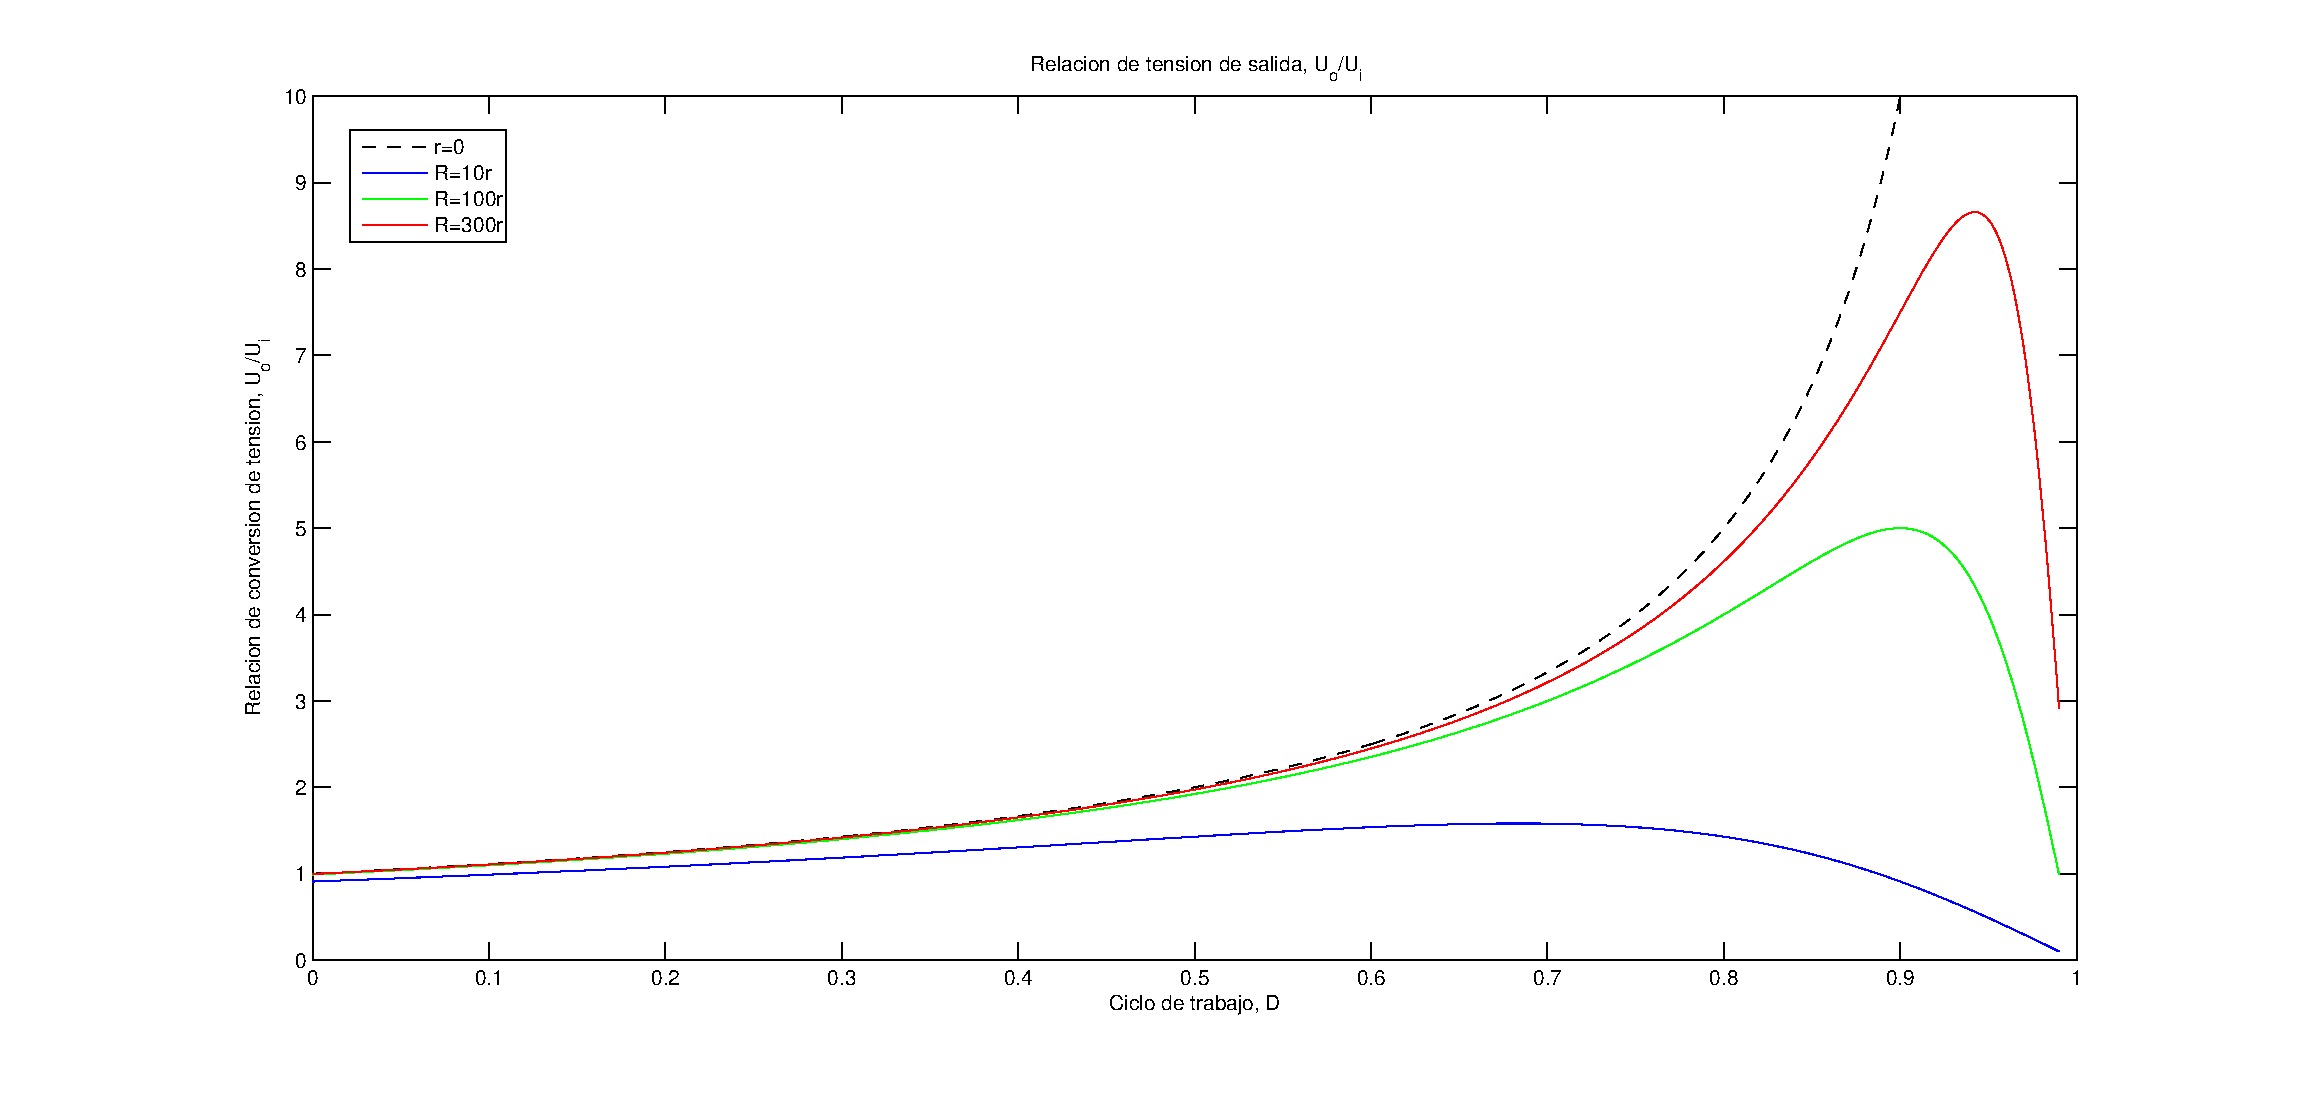
\includegraphics[width=12cm]{gfx/relacion_elevador.eps}
 \caption{Relaciones de tensión del convertidor elevador con diferentes cargas.}
 \label{fig:relacion_elevador}
\end{figure}
\begin{figure}[H]
 \centering
 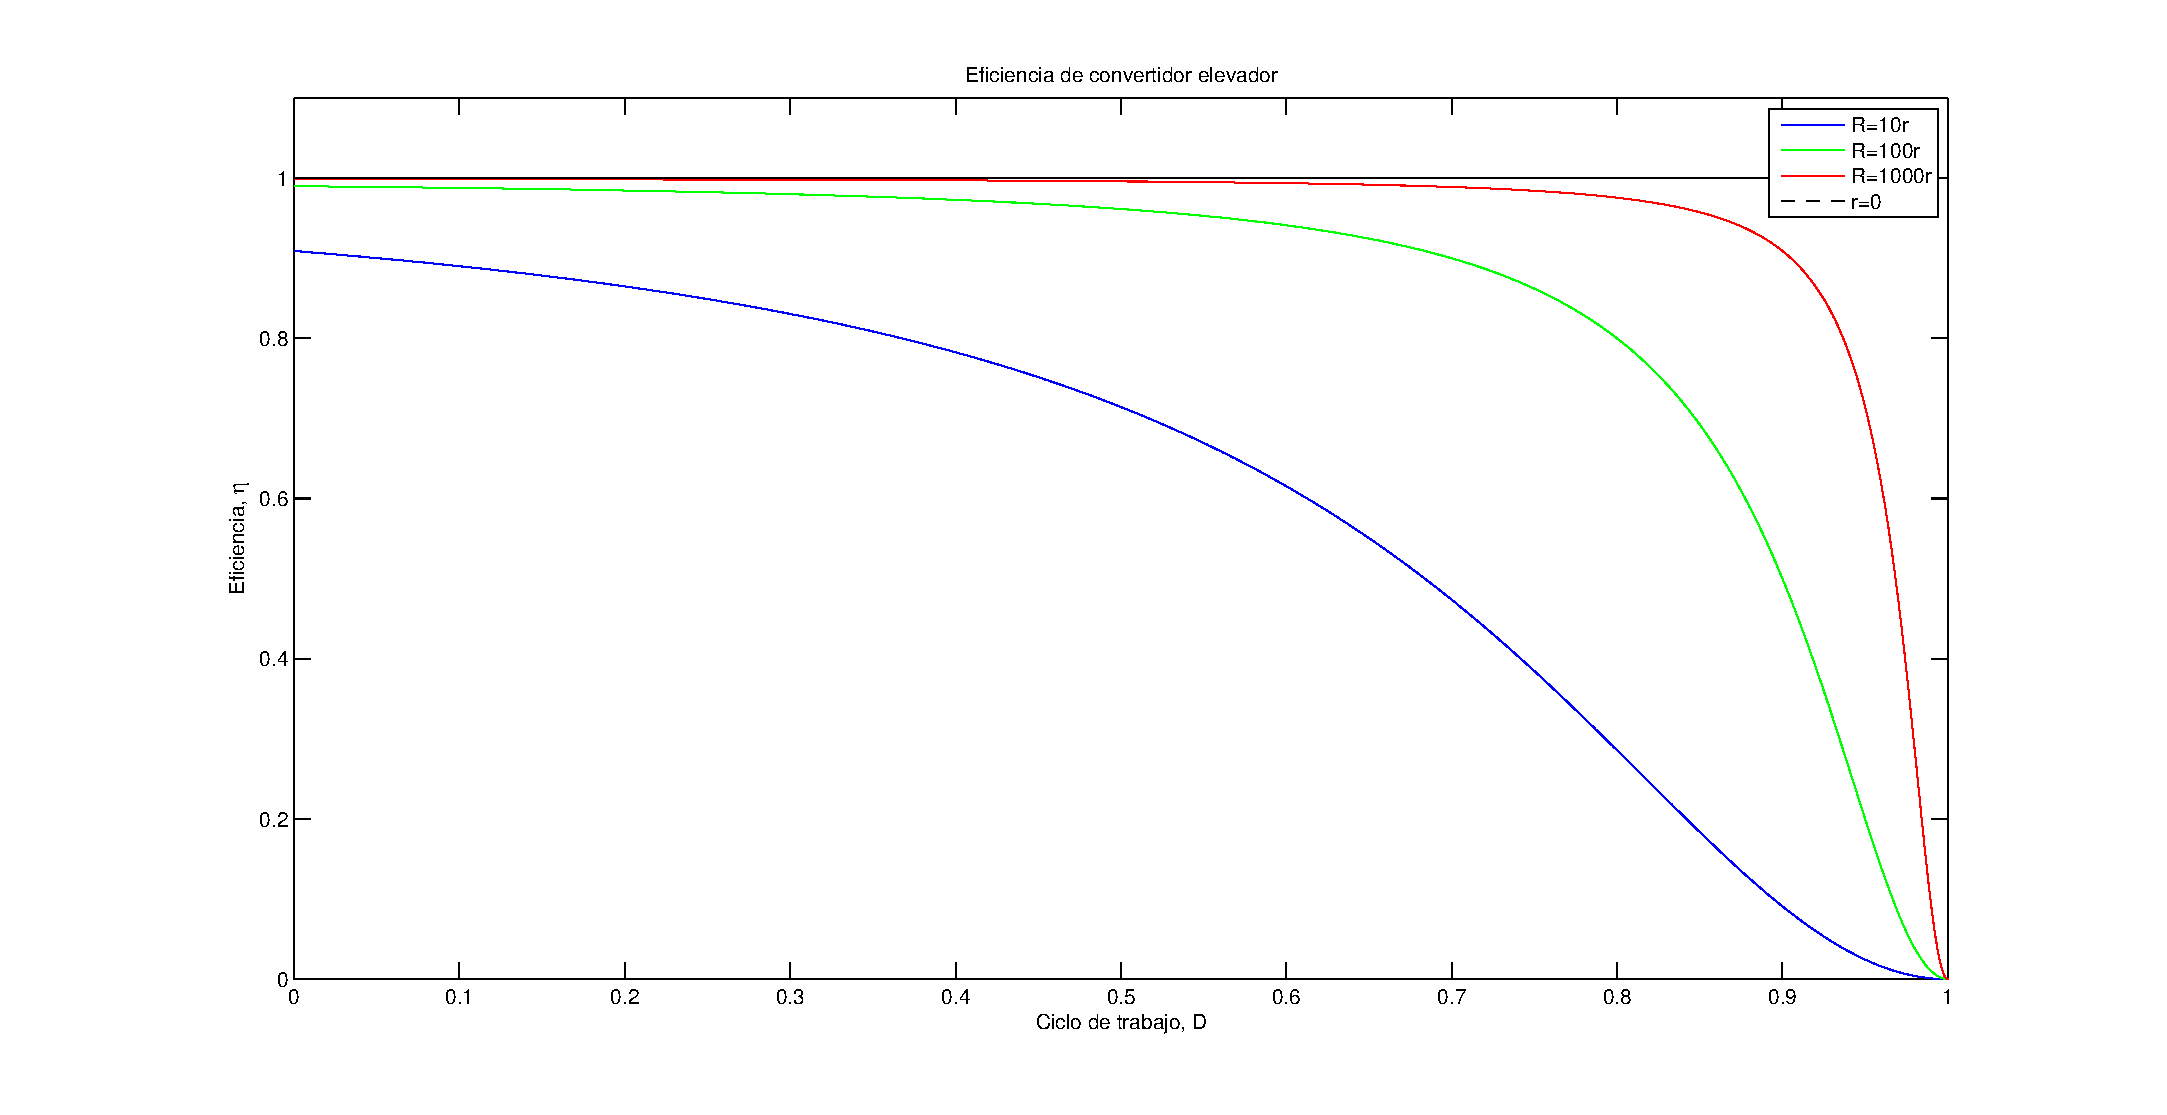
\includegraphics[width=12cm]{gfx/eficiencia_elevador.eps}
 \caption{Eficiencia del convertidor elevador a diferentes cargas.}
 \label{fig:eficiencia_elevador}
\end{figure}
Como el análisis se hace en estado estacionario si se examina la corriente que atraviesa el inductor usando la (\ref{eq:aprox_corriente})
la variación de la corriente es la misma tanto para la llave abierta como cerrada y resulta,
$$\frac{\Delta i_{L,cerrada}}{\Delta t}=\frac{\Delta i_{L,abierta}}{\Delta t}$$
\begin{subequations}
  \begin{equation}
   \Delta i_{L,cerrada}=\frac{U_i}{L}DT_s
  \end{equation}
  \begin{equation}
   \Delta i_{L,abierta}=\frac{U_i-U_o}{L}(1-D)T_s
  \end{equation}
\end{subequations}
A partir la fig. \ref{fig:elevador_CC} puede establecerse un límite entre los dos modos de operación MCC y MCD (modo de conducción discontinua).
Si se observa que al reducir la carga y con ella la corriente media a la salida del convertidor, también disminuye la corriente que atraviesa
el inductor, hay un punto en que $i_L$ se hace $0$. Teniendo en cuenta que la forma de la señal de corriente a través del inductor se aproxima
por una onda triangular se llega al siguiente resultado:
\begin{subequations}
 \begin{equation}
  \bar{i}_{L,min}=\frac{1}{2}\hat{i}_L
 \end{equation}
 \begin{equation}
  \bar{i}_{L,min}=\frac{1}{2}\frac{U_iDT_s}{L}
 \end{equation}
 \begin{equation}
  \bar{i}_{L,min}=\frac{1}{2}\frac{U_oD(1-D)T_s}{L}
 \end{equation}
\end{subequations}
Resulta útil expresar este límite en función de la corriente de carga, puesto que la tensión de salida se pretende mantener constante.
\begin{equation}
 \bar{i}_{o,min}=\frac{U_oT_s}{2L}D(1-D)^2
 \label{eq:limite_corriente_elevador}
\end{equation}
Al inicio del análisis se asumió que el capacitor del filtro de salida era suficientemente grande como para que la variación en la tensión de salida sea despreciable.
Aunque esta aproximación es válida para realizar los cálculos previos, se encuentra presente un pequeño rizado. Si se considera que en la práctica el
capacitor tiene capacidad finita y además posee una resistencia serie parásita (ESR) sobre la cual puede producirse una caída de tensión
puede hallarse una aproximación del valor del rizado de la tensión de salida. Esta variación se puede computar a partir de la variación en la carga del mismo y usando
la ley de ohm, respectivamente. 
Estos efectos pueden sumarse para considerar un caso pesimista del cálculo de la variación de tensión de salida,
$$\Delta U_o < \Delta U_{o,C} + \Delta U_{o,ESR} $$
Que establece una cota a partir de la suma de la variación provocada por la capacidad finita y la presencia de la resistencia parásita.

Para obtener la variación debido a la capacidad se estudia la corriente que atraviesa el capacitor,
$$ i_C=i_L-i_o $$
Para ello se examina la fig. \ref{fig:corriente_capacitor_elevador_MCC} y entonces si la corriente es positiva el capacitor se está cargando, en contraste si es
negativa, ocurre lo contrario. Partiendo de las definiciones de capacidad,
$$ \Delta U_{o,C}=\frac{\Delta Q}{C} $$
La variación de carga se obtiene al aplicar reglas geométricas al área sombreada de la fig. \ref{fig:corriente_capacitor_elevador_MCC}, asumiendo que 
$ I_o < i_{L,min}$,
$$ \Delta Q=I_o DT_s=\frac{U_o}{R}DT $$
Sustituyendo en la expresión anterior se tiene,
$$\Delta U_{o,C}=\frac{U_o DT}{RC}$$
En términos relativos,
\begin{equation}
 \frac{\Delta U_{o,C}}{U_o}=\frac{DT}{RC}
\end{equation}
Para obtener la caída debido a la ESR, simplemente se aplica la ley de ohm usando los valores de resistencia especificados por el fabricante y la variación de
corriente a través del capacitor.
\begin{equation}
 \Delta U_{o,ESR} = \Delta i_C r_C
\end{equation}
Hay que remarcar que muchas veces la caída de tensión debida a la resistencia parásita puede ser mucho mayor que la debida a la capacidad y por ello resulta muy importante
que se utilicen capacitores cuya ESR sea suficientemente baja para no degradar el desempeño del convertidor.

\subsubsection{Exigencias eléctricas en estado estacionario para MCC}

Es muy importante que no se sobrepasen los límites eléctricos para los cuales fueron fabricados los componentes que forman parte del convertidor para no
dañar los componentes. Si se inspeccionan las curvas de estado estacionario, se pueden encontrar las exigencias a las que serán sometidos. 
En el cuadro \ref{tab:exigencias_elevador} se encuentran las solicitaciones eléctricas de interés para cada componente.
\begin{table}[H]
  \centering
  \begin{tabular}{|c|c|c|c|c|}
  \hline 
  Comp. 	& $T_{1}$ & $T_{2}$ & $L$ & $C$\tabularnewline
  \hline 
  \hline 
  $U_{max}$	& $U_{o}$ & $U_{o}$ & $U_{o}-U_{i}$ o $U_{i}$ & $U_{o}$\tabularnewline
  \hline 
  $U_{ef}$	& $U_{o}\sqrt{D}$ & $U_{o}\sqrt{1-D}$ & $\sqrt{U_{i}^{2}D+(U_{i}-U_{o})^{2}(1-D)}$ & $U_{o}$\tabularnewline
  \hline 
  $I_{max}$	& $\frac{I_{o}}{1-D}+\frac{U_{i}D}{2Lf}$ & $\frac{I_{o}}{1-D}+\frac{U_{i}D}{2Lf}$ & $\frac{I_{o}}{1-D}+\frac{U_{i}D}{2Lf}$ & $\frac{I_{o}D}{1-D}+\frac{U_{i}D}{2Lf}$\tabularnewline
  \hline 
  $I_{ef}$ 	&  &  & $\sqrt{\left(\frac{I_{o}}{1-D}\right)^{2}+\frac{1}{3}\left(\frac{U_{i}D}{Lf}\right)^{2}}$ & $I_{o}\sqrt{\frac{D}{1-D}}$\tabularnewline
  \hline 
  \end{tabular}
  \caption{Exigencias eléctricas de los componentes del elevador.}
  \label{tab:exigencias_elevador}
\end{table}
  
\subsubsection{Modo de conducción discontinua}
El siguiente análisis se efectúa para la operación del convertidor con corrientes debajo de los límites de la 
eq. (\ref{eq:limite_corriente_elevador}) es decir en MCD, y de modo similar al que se hizo para MCC se obtendrán las relaciones
de interés examinando las curvas de estado estacionario presentadas en la fig. \ref{fig:estado_estacionario_elevador_MCD}.

\begin{figure}
 \centering
 \subfloat[Tensión de inductor]{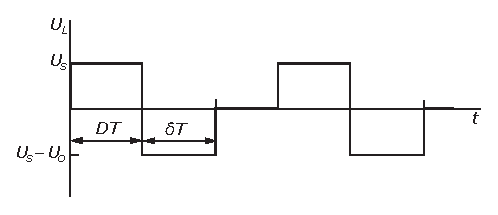
\includegraphics[width=10cm]{gfx/tension_inductor_elevador_MCD.eps}} \\
 \subfloat[Corriente de diodo]{\label{fig:corriente_diodo_elevador_MCD}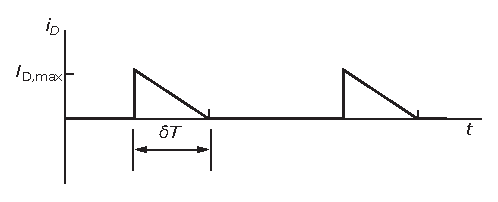
\includegraphics[width=10cm]{gfx/corriente_diodo_elevador_MCD.eps}} \\
 \subfloat[Corriente de inductor]{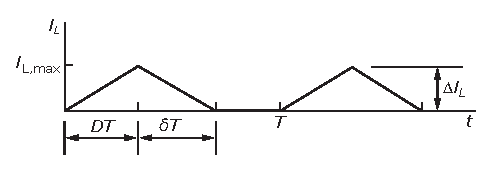
\includegraphics[width=10cm]{gfx/corriente_inductor_elevador_MCD.eps}}
 \caption{Curvas de estado estacionario para el elevador operando en MCC}
 \label{fig:estado_estacionario_elevador_MCD}
\end{figure}

Usando la integral de la tensión en el inductor se obtiene,
$$ U_iD+(U_i-U_o)\delta=0 $$
Siendo $\delta$ el tiempo en sigue habiendo conducción de corriente a través del inductor luego de la apertura del transistor. Esto deriva en las siguientes ecuaciones,

\begin{subequations}
 \begin{equation}
  \frac{U_o}{U_i}=\frac{D+\delta}{\delta}
  \label{eq:relacion_basica}
 \end{equation}
  \begin{equation}
  \frac{I_o}{I_i}=\frac{\delta}{D+\delta}
 \end{equation}
\end{subequations}

Ha aparecido un nuevo parámetro temporal $\delta$ que puede eliminarse usando otras expresiones. Utilizando la fig. \ref{fig:corriente_diodo_elevador_MCD}
se obtiene la corriente continua de salida en términos de los parámetros $D$ y $\delta$:

 $$I_{o}=\frac{U_i D T_s}{2L}\delta=\frac{U_o}{R}$$
 
Se puede despejar $\delta$:

\begin{equation}
 \delta = \frac{U_o}{U_i}\frac{2L}{RDT}
 \label{eq:delta_elevador}
\end{equation}

Sustituyendo la eq. (\ref{eq:delta_elevador}) en la eq. (\ref{eq:relacion_basica}) y resolviendo la ecuación
cuadrática resultante para $\frac{U_o}{U_i}$ se obtiene:

\begin{equation}
 \frac{U_o}{U_i}=\frac{1}{2} \left(1+\sqrt{1+\frac{2D^2RT_s}{L}} \right)
 \label{eq:relacion_elevador_MCD}
\end{equation}

Es posible que el convertidor cambie de modo de operación para una carga fija al variar $D$ ya sea cambiando la referencia de tensión
de salida o debido a variaciones en la tensión de entrada. Esto define intervalos en
la relación de transformación, que dependen del modo de conducción en que opere el equipo. En la 
fig. \ref{fig:caracteristica_elevador_MCD} se muestra un ejemplo de ello.

\begin{figure}[H]
 \centering
 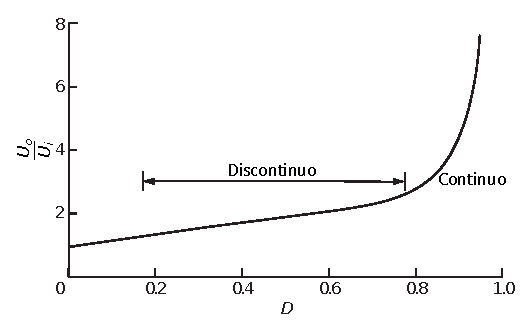
\includegraphics[width=12cm]{gfx/caracteristica_elevador_MCD.eps}
 \caption{Intervalos de modos de conducción para la relación de conversión del elevador.}
 \label{fig:caracteristica_elevador_MCD}
\end{figure}

\subsection{Modelo dinámico}
Las señales de comando del convertidor se obtienen del \emph{hardware} de control que realiza los cálculos necesarios a partir
de los algoritmos con que trabaje. Su estudio y diseño serán abordados en el cap. \ref{ch:control}. Para realizar el diseño, sin
embargo se debe contar con un modelo dinámico. Es por ello que se obtuvo el modelo en variables de estado del sistema considerando 
las pérdidas debidas a los elementos resistivos en serie. El modelo se presenta a continuación,
\[
  \pmb{x}=
  \left(\begin{array}{c}
  i_{L}\\
  u_{C}
  \end{array}\right)
\]

\begin{equation}
\begin{cases}
\pmb{\dot{x}}=\left(\begin{array}{cc}
\frac{-r_{s}}{L} & 0\\
0 & \frac{-1}{RC(1+\frac{r_{C}}{R})}
\end{array}\right)\pmb{x}+\left(\begin{array}{c}
\frac{1}{L}\\
0
\end{array}\right)u_{i}, & 0<t<DT\\
\pmb{\dot{x}}=\left(\begin{array}{cc}
\frac{-(r_{s}(r_{c}+R)+r_{c}R)}{(r_{c}+R)L} & \frac{-1}{(1+\frac{r_{C}}{R})L}\\
\frac{1}{(1+\frac{r_{C}}{R})C} & \frac{-1}{RC(1+\frac{r_{C}}{R})}
\end{array}\right)\pmb{x}+\left(\begin{array}{c}
\frac{1}{L}\\
0
\end{array}\right)u_{i} & DT<t<T
\end{cases}
\end{equation}

\begin{equation}
\begin{cases}
\left(\begin{array}{c}
i_{L}\\
u_{o}
\end{array}\right)=\pmb{y}=\left(\begin{array}{cc}
1 & 0\\
0 & \frac{R}{R+r_{C}}
\end{array}\right)\pmb{x} & 0<t<DT\\
\left(\begin{array}{c}
i_{L}\\
u_{o}
\end{array}\right)=\pmb{y}=\left(\begin{array}{cc}
1 & 0\\
\frac{Rr_{C}}{R+r_{C}} & \frac{R}{R+r_{C}}
\end{array}\right)\pmb{x} & DT<t<T
\end{cases}
\end{equation}

\section{Convertidor reductor}
Este dispositivo sirve para reducir los niveles de tensión de la fuente con la que se lo alimenta. Para el trabajo realizado se dispuso de otro convertidor
elevador idéntico al que se armó para la etapa de adaptación del módulo de pilas de celdas de combustible. Gracias a su diseño fue posible adaptarlo, mediante
ajustes simples, a una topología reductora. El esquemático del circuito reductor se muestra en la fig. \ref{fig:reductor} donde se ha resaltado la
adición de los nuevos componentes sobre el esquemático mostrado en la fig. \ref{fig:elevador}.

Los rangos en los que operará el reductor deben ser adaptables a los del elevador. Esto no supone un problema considerando que uno de los equipos
está  basado en el otro, aunque más adelante se detallan las exigencias a las que será sometido el reductor para asegurar que se mantienen en los rangos
de trabajo permitidos por las hojas de datos de los componentes.

Desde el punto de vista estructural, el convertidor reductor es más sencillo que el elevador ya que la topología se mantiene igual durante cada ciclo de
conmutación. Por lo tanto, la operación de esta configuración puede interpretarse como la aplicación de un filtro pasa-bajos a una señal PWM de amplitud igual 
a la tensión de entrada. De este modo, la tensión devuelta correspondería aproximadamente al valor medio de la señal PWM.

\begin{figure}[H]
 \centering
 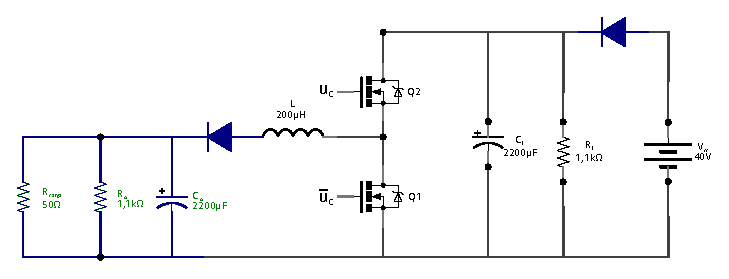
\includegraphics[width=12cm]{gfx/reductor.eps}
 \caption{Esquemático del reductor a partir del circuito del elevador}
 \label{fig:reductor}
\end{figure}

\subsection{Operación en estado estacionario}
Se aplicarán los mismos conceptos vistos en el sec. \ref{sub:elevador_estacionario} para hallar las relaciones que determinan la operación del convertidor
reductor.

\subsubsection{Modo de conducción continua}
Al igual que en el caso del elevador se ha realizado un análisis en estado estacionario del convertidor reductor de cuyos resultados se extrae
suficiente información para decidir sobre la elección de los componentes que serán parte del presente convertidor y para obtener los modelos
a utilizar para el diseño de los algoritmos de control.

En la fig. \ref{fig:reductor_CC} se muestran las curvas para el funcionamiento del convertidor en estado estacionario, para éste caso no es necesario el uso
de las curvas de corriente del diodo.

\begin{figure}
 \centering
 \subfloat[Tensión de inductor]{\label{fig:tension_inductor_reductor_MCC}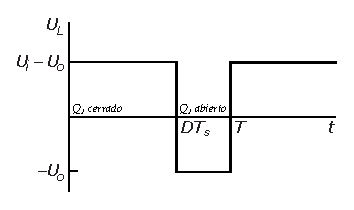
\includegraphics[width=5cm]{gfx/tension_inductor_reductor_MCC.eps}} \quad
 %\subfloat[Corriente de diodo]{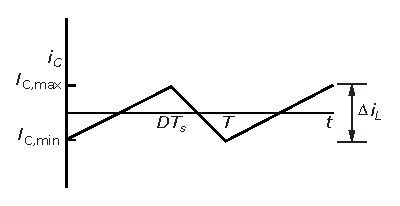
\includegraphics[width=5cm]{gfx/corriente_capacitor_reductor_MCC_simple.eps}} \\
 \subfloat[Corriente de inductor]{\label{fig:corriente_inductor_reductor_MCC}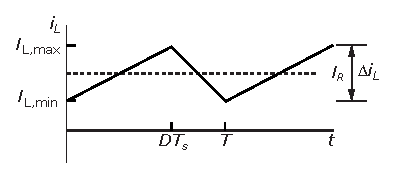
\includegraphics[width=5cm]{gfx/corriente_inductor_reductor_MCC.eps}} \\ \quad
 \subfloat[Corriente de capacitor]{\label{fig:corriente_capacitor_reductor_MCC}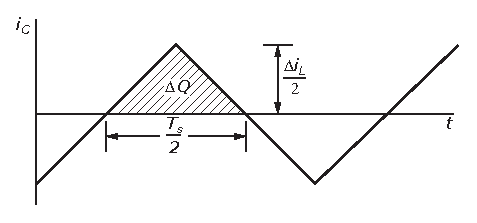
\includegraphics[width=5cm]{gfx/corriente_capacitor_reductor_MCC.eps}}
 \caption{Curvas de estado estacionario para el elevador operando en MCC}
 \label{fig:reductor_CC}
\end{figure}

Mediante los mismos razonamientos utilizados al analizar el elevador se obtienen las relaciones de conversión y los valores límites para la corriente.
A partir de la integral de la tensión del inductor,
$$ (U_i - U_o)D - U_o(1-D)=0 $$
Operando resulta,
\begin{equation}
 \frac{U_o}{U_i}=D
 \label{eq:relacion_reductor}
\end{equation}
Y una vez más, con $P_i=P_o$,
\begin{equation}
 \frac{I_o}{I_i}=\frac{1}{D}
 \label{eq:relacion_corriente_reductor}
\end{equation}

Para analizar el comportamiento de la corriente se asume que la corriente es una onda triangular se usa la (\ref{eq:aprox_corriente})
y se establece que la variación de corriente es igual tanto para el estado cerrado de la llave como el abierto,
\begin{subequations}
  \begin{equation}
   \Delta i_{L,cerrada}=\frac{U_i-U_o}{L}DT_s
  \end{equation}
  \begin{equation}
   \Delta i_{L,abierta}=-\frac{U_o}{L}(1-D)T_s
  \end{equation}
\end{subequations}
Para obtener mayor precisión en los resultados anteriores se consideran los elementos parásitos,
\begin{equation}
 \frac{U_o}{U_i}=\frac{D}{1+\frac{r}{R}}
 \label{eq:relacion_reductor_completa}
\end{equation}
\begin{equation}
 \eta=\frac{P_o}{P_i}=\frac{1}{1+\frac{r}{R}}
 \label{eq:eficiencia_reductor}
\end{equation}
Las ecuaciones \ref{eq:relacion_reductor_completa} y \ref{eq:eficiencia_reductor} reflejan que la relación de conversión
y la eficiencia solo varían por un factor respecto de la relación ideal (en cuyo caso $\eta=1$), además la eficiencia es independiente del ciclo de trabajo,
Esto es favorable ya que no hay necesidad de acotar el rango de trabajo debido a los efectos de los elementos parásitos.

Según la fig. \ref{fig:reductor_CC}, a partir del la variación de corriente por el inductor puede encontrarse el límite entre los dos modos de operación MCC y MCD.

 \begin{equation}
  \bar{i}_{L,min}=\frac{\Delta i_L }{2}= \frac{D T_s(1-D)}{2L}U_i=\frac{T_s(1-D)}{2L}U_o=\bar{i}_{o,min}
  \label{eq:limite_corriente_reductor}
 \end{equation}

Para estudiar las fluctuaciones en la tensión entregada por el convertidor se suman las contribuciones de los efectos de la naturaleza finita de la capacidad
y la ESR. Por lo tanto, a partir de la fig. \ref{fig:corriente_capacitor_reductor_MCC} puede obtenerse la variación en la carga y a partir de esto la variación
en la tensión de salida como se hizo para el caso del elevador.

La variación de carga se obtiene al aplicar reglas geométricas a la fig. \ref{fig:corriente_capacitor_reductor_MCC}:
$$ \Delta Q=\frac{1}{2}\frac{T_s}{2}\frac{\Delta i_L}{2}=\frac{T_s \Delta i_L}{8} $$
Sustituyendo en la expresión anterior:
\begin{equation}
 \Delta U_{o,C}=\frac{T_s \Delta i_L}{8C}=\frac{U_o T_s (1-D)}{8LC}
\end{equation}
\begin{equation}
 \frac{\Delta U_{o,C}}{U_o}=\frac{T_s (1-D)}{8LC}
\end{equation}
En cuanto al efecto de la resistencia parásita se aplica la ley de omh como se hizo en el caso anterior.

\subsubsection{Exigencias eléctricas en estado estacionario para MCC}

Se ha realizado un análisis en estado estacionario del Convertidor Reductor de cuyo análisis se extraerá
suficiente información para decidir sobre la elección de los componentes que serán parte del presente convertidor.
\begin{table}[H]
  \centering
  \begin{tabular}{|c|c|c|c|c|}
  \hline 
  Comp. & $T_{1}$ & $T_{2}$ & $L$ & $C$\tabularnewline
  \hline 
  \hline 
  $U_{max}$ & $U_{o}$ & $U_{o}$ & $U_{o}-U_{i}$ o $U_{o}$ & $U_{o}$\tabularnewline
  \hline 
  $U_{ef}$& $U_{o}\sqrt{1-D}$ & $U_{o}\sqrt{D}$ & $\sqrt{(U_{i}-U_{o})^{2}D+U_{o}^{2}(1-D)}$ & $U_{o}$\tabularnewline
  \hline 
  $I_{max}$ & $I_{o}+\frac{U_{o}(1-D)}{2Lf}$ & $I_{o}+\frac{U_{o}(1-D)}{2Lf}$ & $I_{o}+\frac{U_{o}(1-D)}{2Lf}$ & $\frac{U_{o}(1-D)}{2Lf}$\tabularnewline
  \hline 
  $I_{ef}$ &  &  & $\sqrt{I_{o}^{2}+\frac{1}{3}\left(\frac{U_{o}(1-D)}{Lf}\right)^{2}}$ & $\frac{U_{o}(1-D)}{\sqrt{3}Lf}$\tabularnewline
  \hline 
  \end{tabular}
  \caption{Exigencias eléctricas de los componentes del reductor.}
  \label{tab:exigencias_reductor}
\end{table}
\subsubsection{Modo de conducción discontinua}
Cuando la corriente disminuye por debajo del margen de la eq. (\ref{eq:limite_corriente_reductor} el dispositivo entra conducción discontinua y cuando eso ocurre, las
características cambian al igual que ocurre para el elevador. Con ayuda de las figs. \ref{fig:estado_estacionario_reductor_MCD} se obtienen los desarrollos presentados 
a continuación.

\begin{figure}
 \centering
 \subfloat[Tensión de inductor]{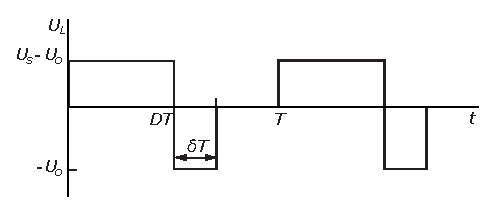
\includegraphics[width=10cm]{gfx/tension_inductor_reductor_MCD.eps}} \\
 \subfloat[Corriente de diodo]{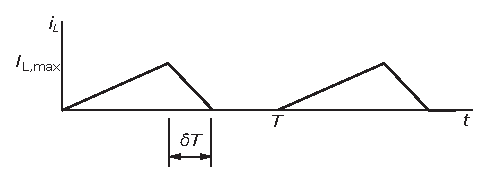
\includegraphics[width=10cm]{gfx/corriente_inductor_reductor_MCD.eps}} \\
 \subfloat[Corriente de inductor]{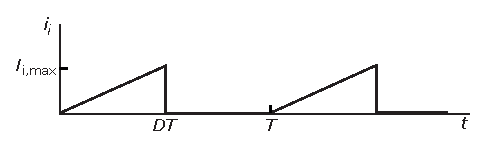
\includegraphics[width=10cm]{gfx/corriente_fuente_reductor_MCD.eps}}
 \caption{Curvas de estado estacionario para el elevador operando en MCC}
 \label{fig:estado_estacionario_reductor_MCD}
\end{figure}
Estudiando nuevamente la integral de la tensión en el inductor,
$$ (U_i-U_o)D-U_o\delta=0 $$
Reordenando se tiene,
\begin{equation}
 \frac{U_o}{U_i}=\frac{D}{D+\delta}
 \label{eq:relacion_reductor_MCD}
\end{equation}
Por otra parte, para la corriente,
\begin{equation}
 \Delta i_{L}=\frac{U_i-U_o}{L}DT_s=\frac{U_o\delta T_s}{L}
\end{equation}
Asumiendo constante la tensión de salida,
\begin{equation}
 I_o=\frac{U_o}{R}=\frac{1}{2}\Delta i_L(D+\delta)=\frac{1}{2}\frac{U_i-U_o}{L}DT_s(D+\delta)
\end{equation}
Usando (\ref{eq:relacion_reductor_MCD}) y reordenando se llega a una ecuación de segundo grado, de cuyas soluciones, se usa la que produce valores positivos,
\begin{equation}
 \delta=\frac{-D+\sqrt{D^2+\frac{8L}{RT}}}{2}
\end{equation}
Sustituyendo en la eq. (\ref{eq:relacion_reductor_MCD}),
\begin{equation}
 \frac{U_o}{U_i}=\frac{2D}{D+\sqrt{D^2+\frac{8L}{RT}}}
\end{equation}
Si se fija la corriente de carga puede provocar que la característica del reductor adopte un comportamiento
mixto respecto a los modos de conducción operando en gran parte del rango del ciclo de trabajo
($D$), esto quiere decir que para estos casos el convertidor puede conmutar entre MCC y MCD. Esto se ilustra en la 
fig. \ref{fig:caracteristica_reductor_MCD}.
\begin{figure}
 \centering
 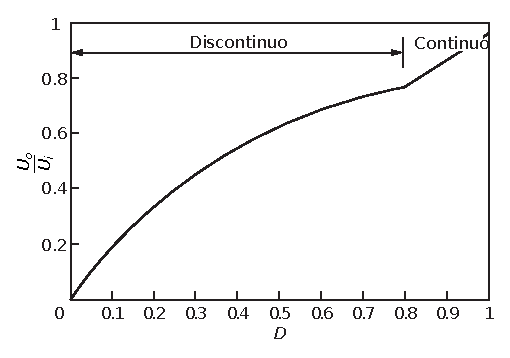
\includegraphics[width=12cm]{gfx/caracteristica_reductor_MCD.eps}
 \caption{Intervalos de modos de conducción para la relación de conversión del reductor.}
 \label{fig:caracteristica_reductor_MCD}
\end{figure}
\subsection{Modelo dinámico}
En esta instancia se presenta el modelo del sistema dinámico del reductor.

\begin{equation}
  \pmb{x}=
  \left(\begin{array}{c}
  i_{L}\\
  u_{C}
  \end{array}\right)
\end{equation}
  
\begin{equation}
  \begin{cases}
  \pmb{\dot{x}}=\left(\begin{array}{cc}
		      \frac{-(r_{s}(r_{c}+R)+r_{c}R)}{(r_{c}+R)L} 	& \frac{-1}{(1+\frac{r_{C}}{R})L}\\
		      \frac{1}{(1+\frac{r_{C}}{R})C} 				& \frac{-1}{RC(1+\frac{r_{C}}{R})}
  \end{array}\right)\pmb{x}+\left(\begin{array}{c}
				  \frac{1}{L}\\
				  0
  \end{array}\right) & 0<t<DT\\
  \pmb{\dot{x}}=\left(\begin{array}{cc}
			\frac{-(r_{s}(r_{c}+R)+r_{c}R)}{(r_{c}+R)L} 	& \frac{-1}{(1+\frac{r_{C}}{R})L}\\
			\frac{1}{(1+\frac{r_{C}}{R})C} 				& \frac{-1}{RC(1+\frac{r_{C}}{R})}
  \end{array}\right)\pmb{x}+\left(\begin{array}{c}
				  0\\
				  0
  \end{array}\right) & DT<t<T
  \end{cases}
\end{equation}


\begin{equation}
  \begin{cases}
  \left(\begin{array}{c}
  i_{L}\\
  u_{o}
  \end{array}\right)=\pmb{y}=\left(\begin{array}{cc}
  1 & 0\\
  \frac{Rr_{C}}{R+r_{C}} & \frac{R}{R+r_{C}}
  \end{array}\right)\pmb{x} & DT<t<T\\
  \left(\begin{array}{c}
  i_{L}\\
  u_{o}
  \end{array}\right)=\pmb{y}=\left(\begin{array}{cc}
  1 & 0\\
  \frac{Rr_{C}}{R+r_{C}} & \frac{R}{R+r_{C}}
  \end{array}\right)\pmb{x} & DT<t<T
  \end{cases}
\end{equation}

Este sistema esta siempre definido por la misma matriz de estados simplificando su análisis, en efecto, el cambio se produce solo sobre
excitación. Por lo tanto puede pensarse que la salida es una señal de pulsos de ancho modulado cuya amplitud corresponde a la tensión de entrada. 

\section{Detalles técnicos de los convertidores utilizados}
Si bien se desarrolló de forma genérica la teoría general de convertidores, en esta sección se presentarán las especificaciones bajo las cuales funcionan
los equipos armados usando la teoría expuesta.

\begin{table}[H]
  \centering
  \begin{tabular}{|c|>{\centering}p{2.5cm}|c|c|c|c|c|}
  \hline 
  Componente & $R_{s}$ & $L$ & $C$ & $I_{ef}$ & $\hat{I}$ & $\hat{U}$\tabularnewline
  \hline 
  \hline 
  Inductor   & $21m\Omega$ $(DC)$ $33m\Omega$ $(AC)$ & $200\mu H$ & - & $15A$ & $16,7A$ & -\tabularnewline
  \hline 
  Capacitor & $50m\Omega$ &  - & $2,2mF$ & $8A$ & - & $100V$\tabularnewline
  \hline 
  Transistor(IRFP-250) & $85m\Omega$ $(r_{T})$ $200m\Omega$ $(r_{D})$ & - & - & $30A$ & $120A$ & $200V$\tabularnewline
  \hline 
  \end{tabular}
  \caption{Especificaciones de los componentes utilizados}
  \label{tab:especificaciones}
\end{table}

\subsection{Convertidor elevador}
El \emph{hardware} correspondiente al elevador construido ha sido diseñado para actuar bajo las siguientes condiciones de operación:

\begin{table}[H]
  \centering
  \begin{tabular}{|c|c|}
  \hline 
  Magnitud & \tabularnewline
  \hline 
  \hline 
  Potencia neta nominal & 300W\tabularnewline
  \hline 
  Tensión de salida nominal & 60V\tabularnewline
  \hline 
  Corriente de salida nominal & 5A\tabularnewline
  \hline 
  Tensión máxima de entrada & 50V\tabularnewline
  \hline 
  Tensión máxima de salida & 100V\tabularnewline
  \hline 
  Corriente máxima en la entrada & 18,5A\tabularnewline
  \hline 
  Corriente máxima en la salida & 5,5A\tabularnewline
  \hline 
  Frecuencia de conmutación & 20kHz\tabularnewline
  \hline 
  Variación de corriente ($ \Delta i_L $) & 3,75A\tabularnewline
  \hline
  \end{tabular}
  \caption{Condiciones de operación para el elevador}
  \label{tab:especificaciones_elevador}
\end{table}

Los límites de las magnitudes anteriores sirvieron de referencia para los ajustes realizados sobre el
acondicionamiento de los circuitos de medida. Estos valores corresponden a los valores máximos según el
circuito acondicionamiento de señales, teniendo en cuenta los rangos
de los sensores involucrados.

Por otro lado es necesario considerar las exigencias que tendrán los componentes operando bajo las condiciones anteriores. Esto se verifica usando el
análisis del circuito en condiciones de estado estacionario. Usando la información listada en el cuadro \ref{tab:especificaciones_elevador} 
junto con las expresiones en el cuadro \ref{tab:exigencias_elevador} se obtienen
las solicitaciones eléctricas a las que serán sometidos los componentes del convertidor elevador que se muestran en el cuadro \ref{tab:solicitaciones_elevador}.

\begin{table}[H]
  \centering
 \begin{tabular}{|c|c|c|c|c|}
  \hline 
  Componente & $T_{1}$ & $T_{2}$ & $L$ & $C$\tabularnewline
  \hline 
  \hline 
  Tensión pico & $60V$ & $60V$ & $<60V$ & $60V$\tabularnewline
  \hline 
  Tensión eficaz & $43V$ & $43V$ & $30V$ & $60V$\tabularnewline
  \hline 
  Corriente pico & $8A$ & $8A$ & $8A$ & $6A$\tabularnewline
  \hline 
  Corriente eficaz &  &  & $9A$ & $4A$\tabularnewline
  \hline 
 \end{tabular}
 \caption{Requerimientos a los componentes del elevador}
 \label{tab:solicitaciones_elevador}
\end{table}

Se han realizado simulaciones para validar el estudio utilizando los valores reales de los componentes con los que se armaron las placas.
En la fig. \ref{fig:boostCC} se presentan las curvas de operación en estado estacionario para el convertidor elevador operando a $D=75\%$ y una corriente de
aproximadamente $6A$.
También se han ejecutado simulaciones para las condiciones de trabajo en MCD que se muestran en la fig. \ref{fig:boostCD} en las que se ha fijado
un ciclo de trabajo de $D=25\%$ y una corriente de carga de $1.8A$.
\begin{figure}
 \centering
 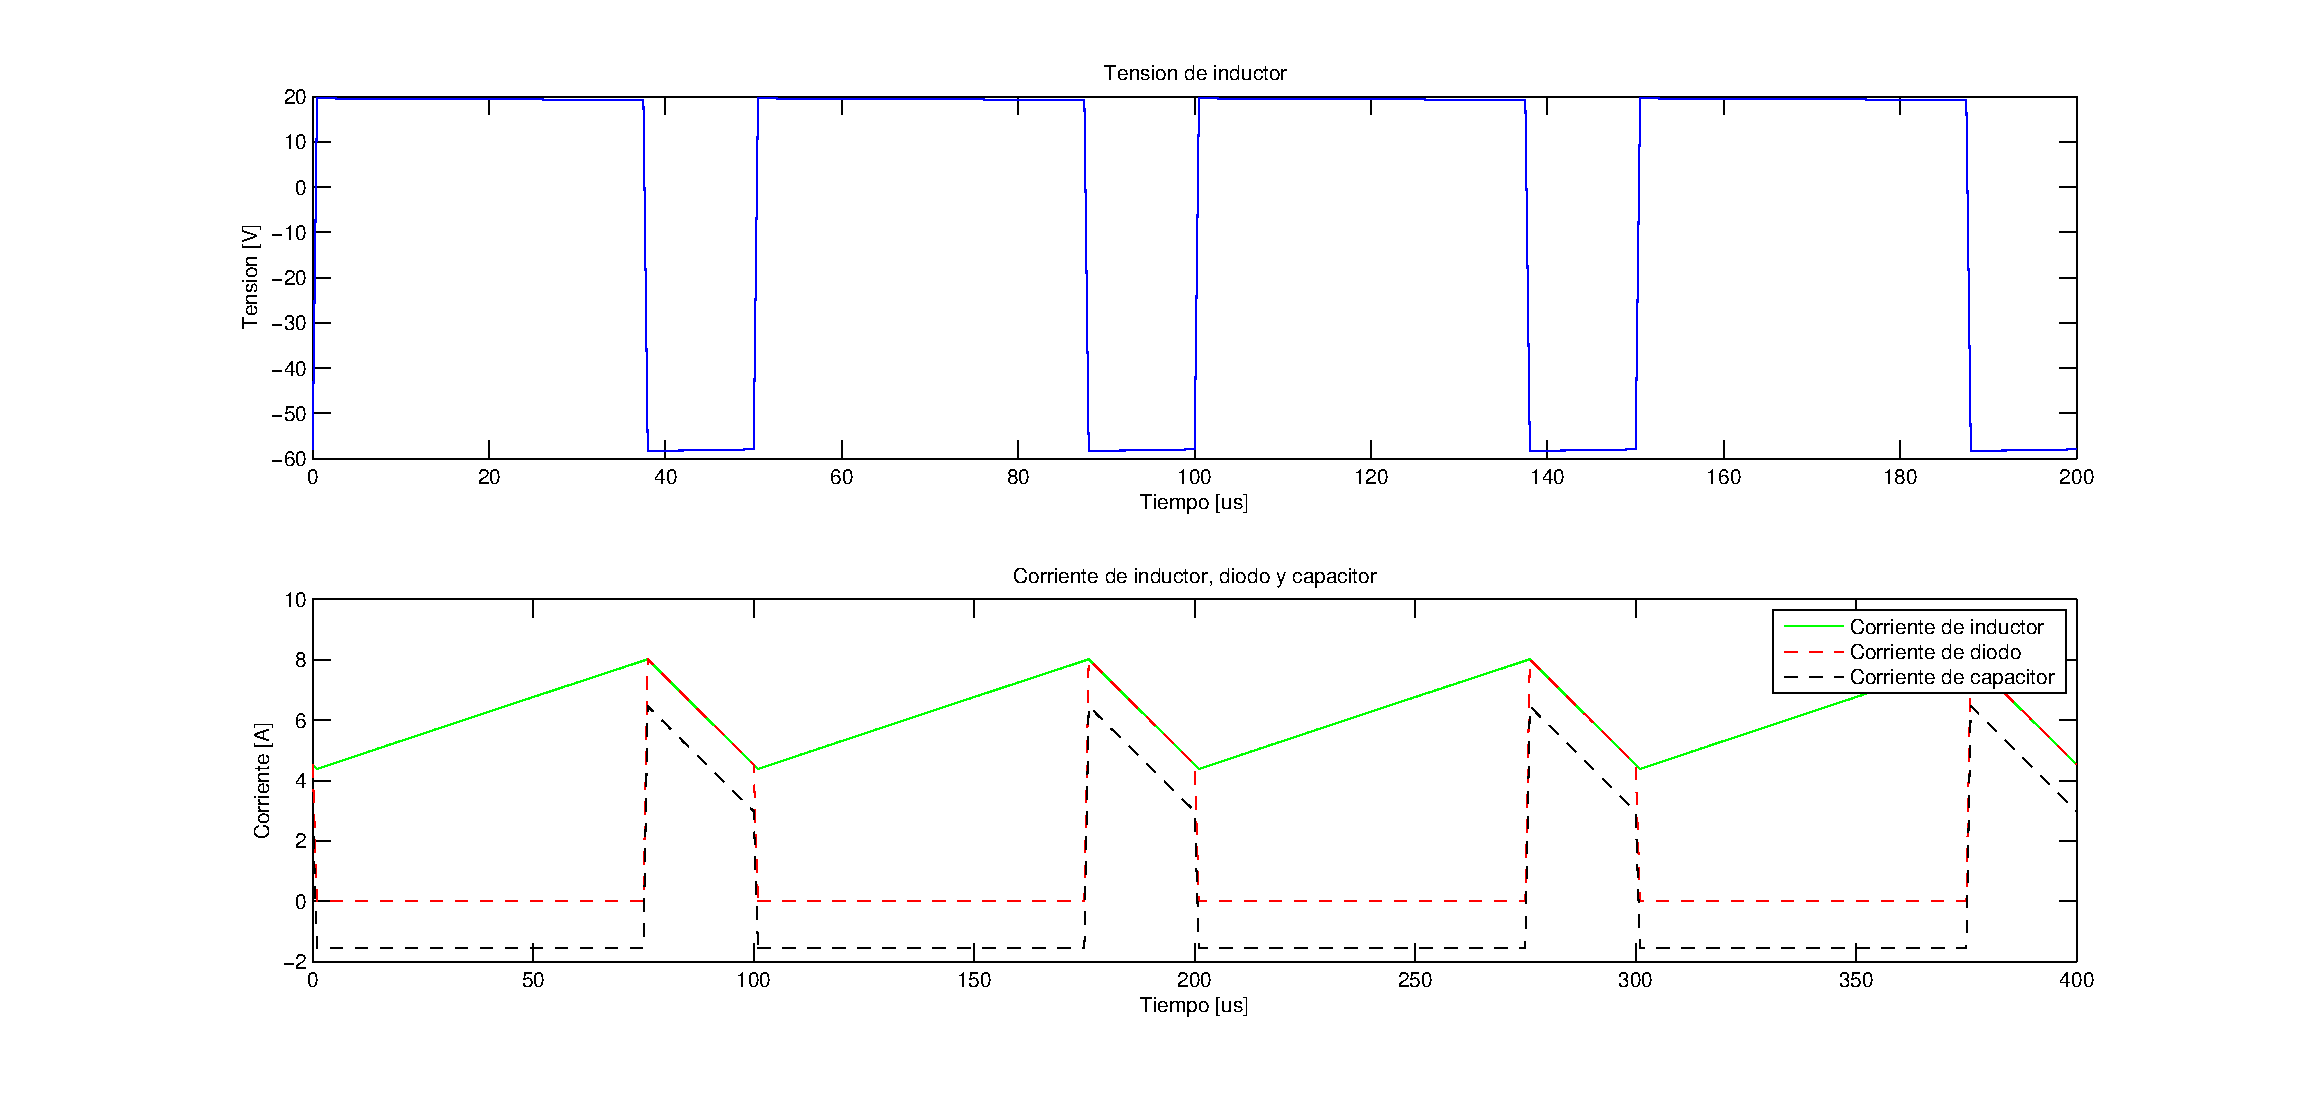
\includegraphics[width=12cm]{gfx/boostCC.eps}
 \caption{Convertidor elevador operando en MCC}
 \label{fig:boostCC}
\end{figure}

\begin{figure}
 \centering
 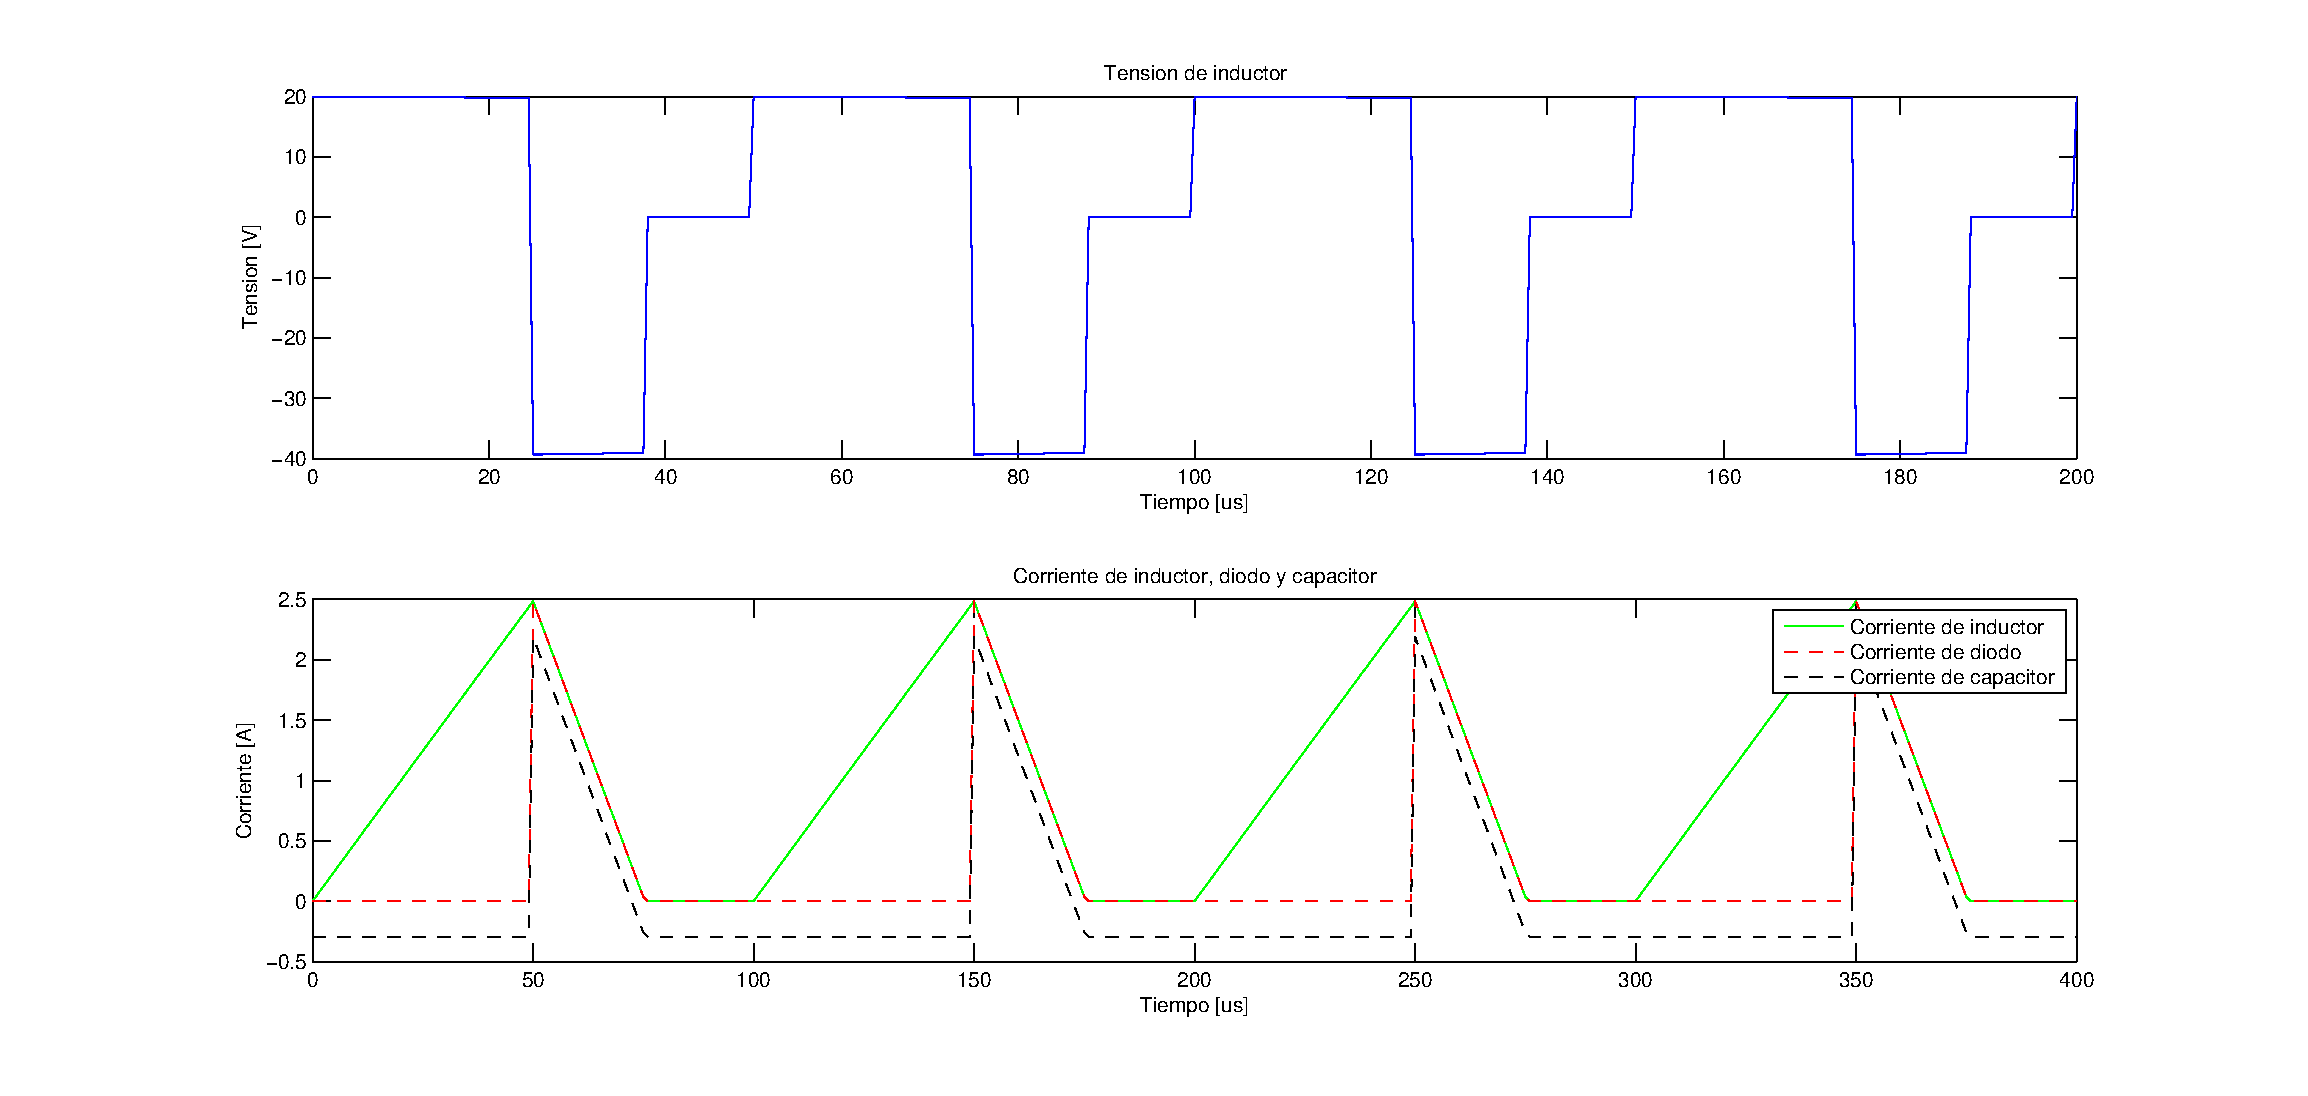
\includegraphics[width=12cm]{gfx/boostCD.eps}
 \caption{Convertidor elevador operando en MCD}
 \label{fig:boostCD}
\end{figure}

\subsection{Convertidor reductor}
A partir del esquemático y las magnitudes de trabajo del elevador se pueden inferir las condiciones de operación para el reductor, que
se listan en el siguiente cuadro:

\begin{table}[H]
  \centering
  \begin{tabular}{|c|c|}
  \hline 
  Magnitud & \tabularnewline
  \hline 
  \hline 
  Potencia neta nominal & 300W\tabularnewline
  \hline 
  Tensión de salida nominal & 30V\tabularnewline
  \hline 
  Corriente de salida nominal & 10A\tabularnewline
  \hline 
  Tensión máxima de entrada & 50V\tabularnewline
  \hline 
  Tensión máxima de salida & 50V\tabularnewline
  \hline 
  Corriente máxima en la entrada & 10A\tabularnewline
  \hline 
  Corriente máxima en la salida & 15A\tabularnewline
  \hline 
  Frecuencia de conmutación & 20kHz\tabularnewline
  \hline 
  Variación de corriente ($ \Delta i_L $) & 3A\tabularnewline
  \hline
  \end{tabular}
  \caption{Condiciones de operación para el elevador}
  \label{tab:especificaciones_reductor}
\end{table}

Al igual que para el convertidor elevador se pueden obtener las exigencias eléctricas a las que se someten los componentes del reductor, según
el análisis de estado estacionario del mismo. Estos datos se han calculado considerando la utilización de los mismos componentes que los del
elevador. La tabla \ref{tab:solicitaciones_reductor} muestra esto.

\begin{table}[H]
  \centering
  \begin{tabular}{|c|c|c|c|c|}
  \hline 
  Componente & $T_{1}$ & $T_{2}$ & $L$ & $C$\tabularnewline
  \hline 
  \hline 
  Tensión pico & $40V$ & $40V$ & $<40V$ & $40V$\tabularnewline
  \hline 
  Tensión eficaz & $28V$ & $28V$ & $20V$ & $40V$\tabularnewline
  \hline 
  Corriente pico & $15A$ & $15A$ & $15A$ & $1,2A$\tabularnewline
  \hline 
  Corriente eficaz &  &  & $15A$ & $1,4A$\tabularnewline
  \hline 
  \end{tabular}
  \caption{Requerimientos a los componentes del reductor}
  \label{tab:solicitaciones_reductor}
 \end{table}
 
A fin de obtener una referencia del funcionamiento cuantitativo del convertidor se han ejecutado algunas simulaciones
con ciclos de trabajo y cargas fijas, tal como se realizó para el elevador. Para el caso de la operación en modo de 
conducción continua las curvas obtenidas se muestran en la fig. \ref{fig:buckCC} que opera con un ciclo de trabajo de
$D=75\%$ y entregando aproximadamente $1A$. En contraste, la fig. \ref{fig:buckCD} muestra las curvas del convertidor
trabajando en MCD con un ciclo de trabajo de $D=25\%$ y una carga aproximada de $600mA$.
 
\begin{figure}[H]
 \centering
 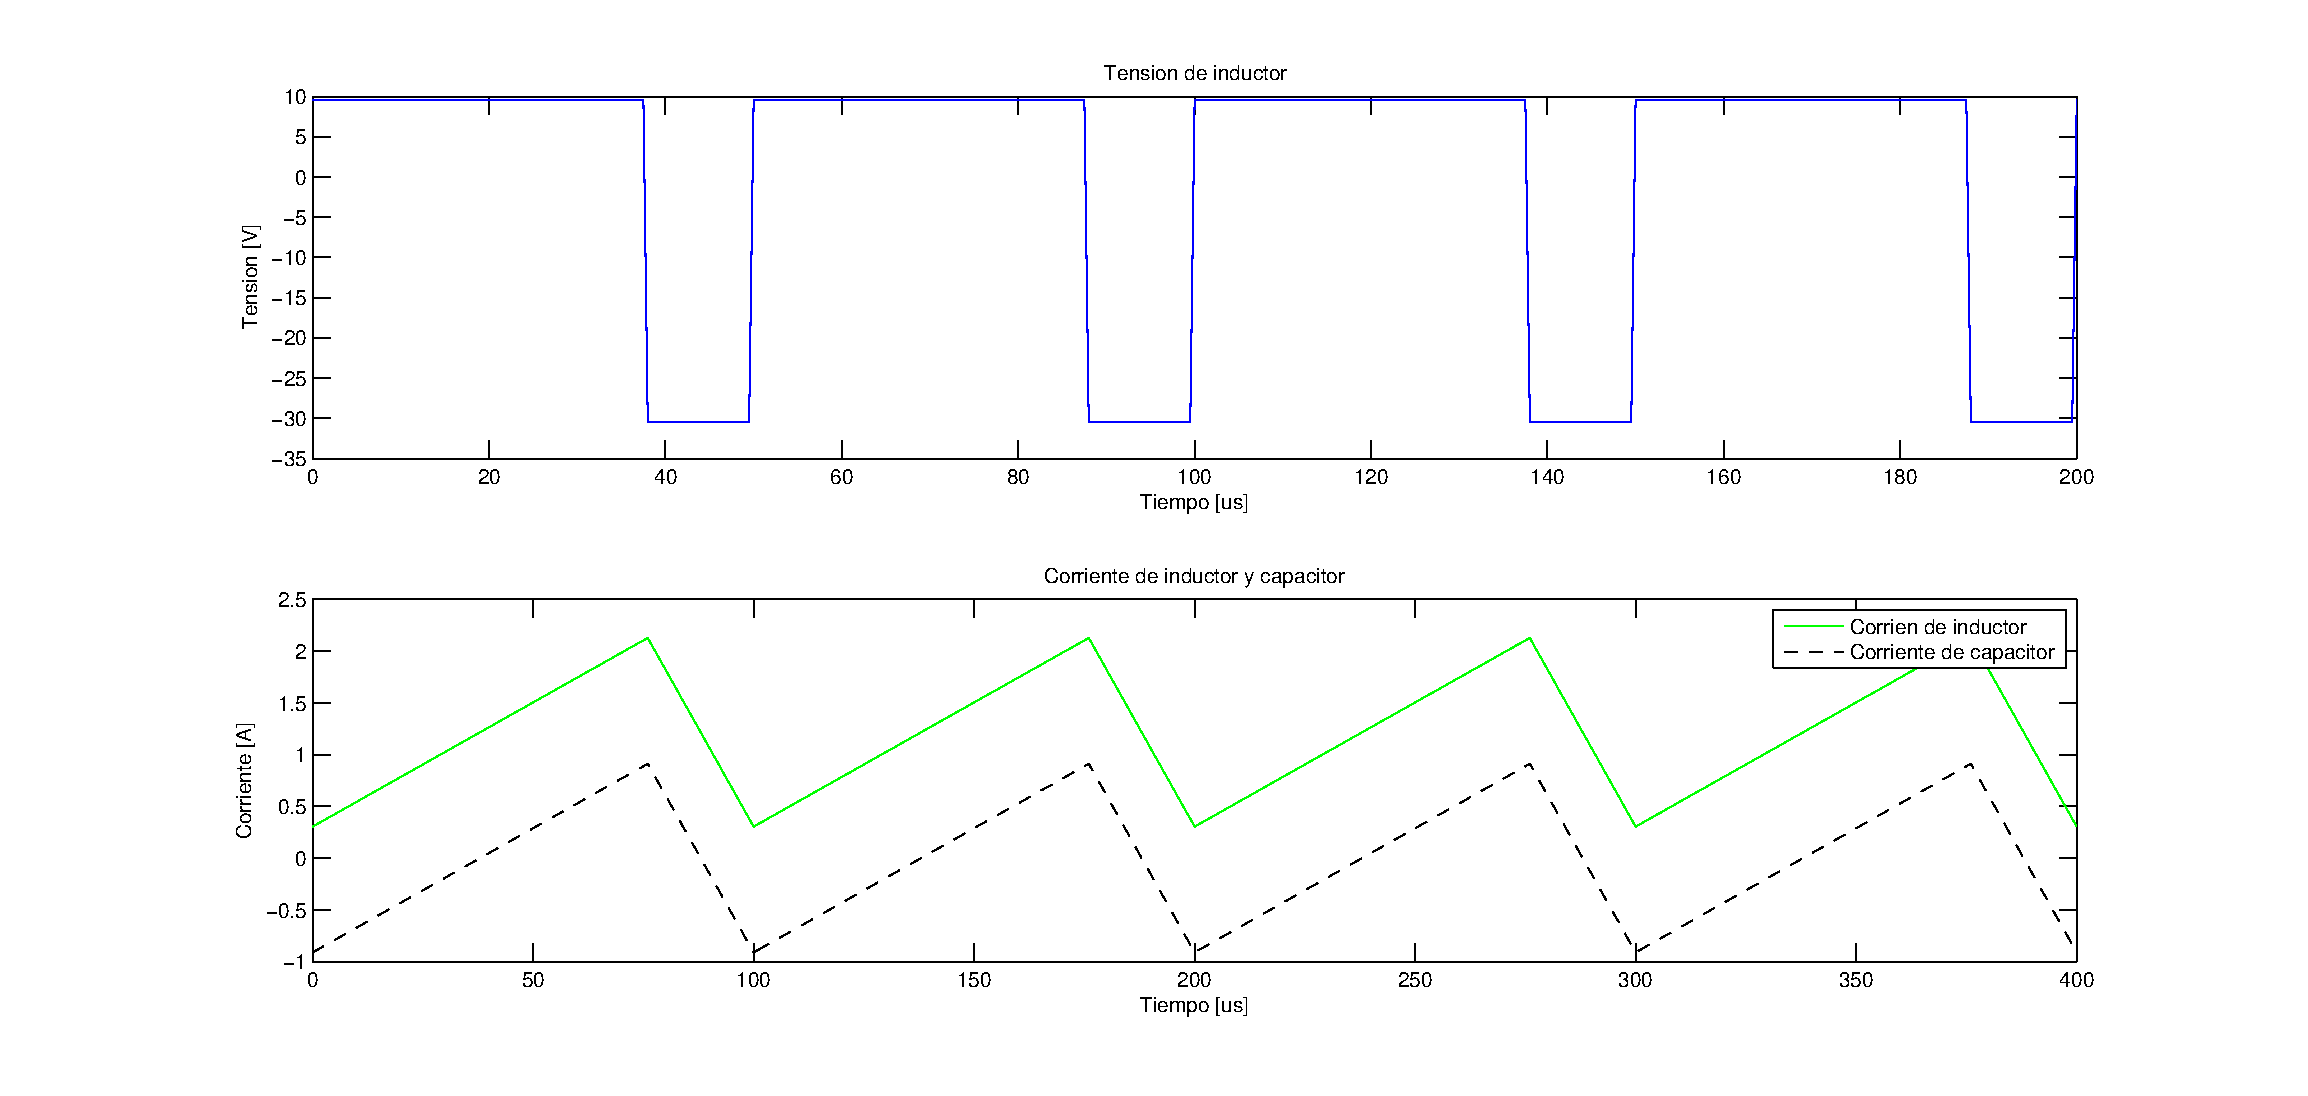
\includegraphics[width=12cm]{gfx/buckCC.eps}
 \caption{Convertidor reductor operando en MCC}
 \label{fig:buckCC}
\end{figure}

\begin{figure}[H]
 \centering
 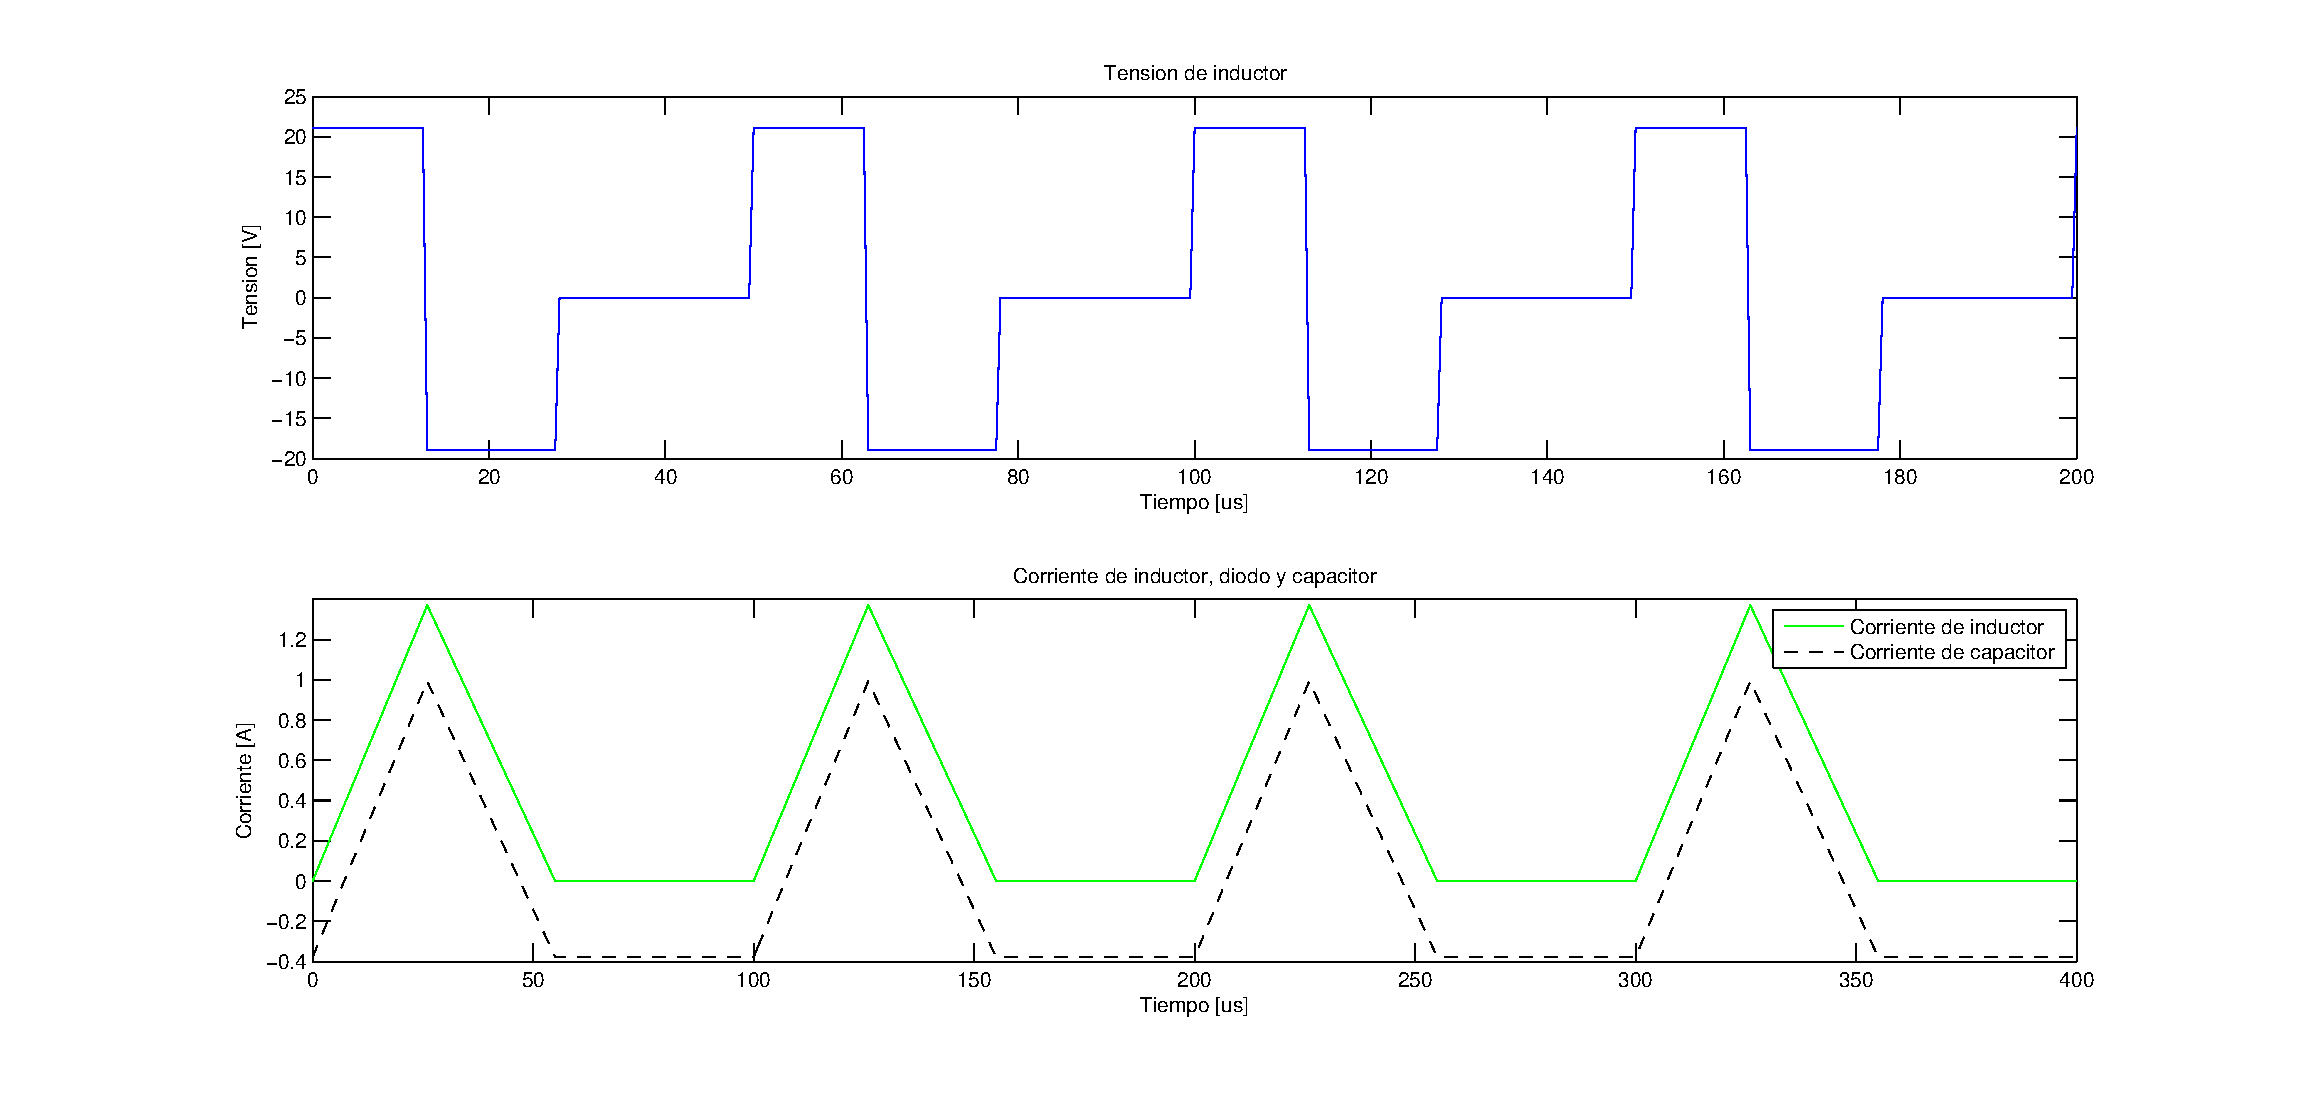
\includegraphics[width=12cm]{gfx/buckCD.eps}
 \caption{Convertidor reductor operando en MCD}
 \label{fig:buckCD}
\end{figure}

\section{Comentarios}
A lo largo del capítulo se han introducido los conceptos elementales que definen los rasgos fundamentales de los convertidores conmutados y
se ha mostrado cómo se manifiestan el comportamiento de los convertidores mediante la variación de los parámetros que los definen. Esta
información será de vital importancia para el desarrollo que sigue, orientado al control de estos dispositivos. 

Los convertidores de potencia DC-DC se controlan a través del estado de sus llaves. Su comportamiento y desempeño esta
fuertemente asociado a los parámetros temporales que surgen del modo en que se operan estas llaves, y estos resultados se utilizaron para el 
planteo de los algoritmos explicados en el capitulo siguiente.

Además, se presentaron las características prácticas generales que detallan los componentes empleados en el armado de las placas y del mismo
modo, los cambios realizados para la obtención de la plataforma utilizada para el emulador.
\end{comment}
